% Options for packages loaded elsewhere
\PassOptionsToPackage{unicode}{hyperref}
\PassOptionsToPackage{hyphens}{url}
%
\documentclass[
]{article}
\usepackage{amsmath,amssymb}
\usepackage{lmodern}
\usepackage{iftex}
\ifPDFTeX
  \usepackage[T1]{fontenc}
  \usepackage[utf8]{inputenc}
  \usepackage{textcomp} % provide euro and other symbols
\else % if luatex or xetex
  \usepackage{unicode-math}
  \defaultfontfeatures{Scale=MatchLowercase}
  \defaultfontfeatures[\rmfamily]{Ligatures=TeX,Scale=1}
\fi
% Use upquote if available, for straight quotes in verbatim environments
\IfFileExists{upquote.sty}{\usepackage{upquote}}{}
\IfFileExists{microtype.sty}{% use microtype if available
  \usepackage[]{microtype}
  \UseMicrotypeSet[protrusion]{basicmath} % disable protrusion for tt fonts
}{}
\makeatletter
\@ifundefined{KOMAClassName}{% if non-KOMA class
  \IfFileExists{parskip.sty}{%
    \usepackage{parskip}
  }{% else
    \setlength{\parindent}{0pt}
    \setlength{\parskip}{6pt plus 2pt minus 1pt}}
}{% if KOMA class
  \KOMAoptions{parskip=half}}
\makeatother
\usepackage{xcolor}
\IfFileExists{xurl.sty}{\usepackage{xurl}}{} % add URL line breaks if available
\IfFileExists{bookmark.sty}{\usepackage{bookmark}}{\usepackage{hyperref}}
\hypersetup{
  pdftitle={Researching the Factors Behind the Pollution in Bangkok, Thailand},
  pdfauthor={Jieyuan Kan},
  hidelinks,
  pdfcreator={LaTeX via pandoc}}
\urlstyle{same} % disable monospaced font for URLs
\usepackage[margin=1in]{geometry}
\usepackage{color}
\usepackage{fancyvrb}
\newcommand{\VerbBar}{|}
\newcommand{\VERB}{\Verb[commandchars=\\\{\}]}
\DefineVerbatimEnvironment{Highlighting}{Verbatim}{commandchars=\\\{\}}
% Add ',fontsize=\small' for more characters per line
\usepackage{framed}
\definecolor{shadecolor}{RGB}{248,248,248}
\newenvironment{Shaded}{\begin{snugshade}}{\end{snugshade}}
\newcommand{\AlertTok}[1]{\textcolor[rgb]{0.94,0.16,0.16}{#1}}
\newcommand{\AnnotationTok}[1]{\textcolor[rgb]{0.56,0.35,0.01}{\textbf{\textit{#1}}}}
\newcommand{\AttributeTok}[1]{\textcolor[rgb]{0.77,0.63,0.00}{#1}}
\newcommand{\BaseNTok}[1]{\textcolor[rgb]{0.00,0.00,0.81}{#1}}
\newcommand{\BuiltInTok}[1]{#1}
\newcommand{\CharTok}[1]{\textcolor[rgb]{0.31,0.60,0.02}{#1}}
\newcommand{\CommentTok}[1]{\textcolor[rgb]{0.56,0.35,0.01}{\textit{#1}}}
\newcommand{\CommentVarTok}[1]{\textcolor[rgb]{0.56,0.35,0.01}{\textbf{\textit{#1}}}}
\newcommand{\ConstantTok}[1]{\textcolor[rgb]{0.00,0.00,0.00}{#1}}
\newcommand{\ControlFlowTok}[1]{\textcolor[rgb]{0.13,0.29,0.53}{\textbf{#1}}}
\newcommand{\DataTypeTok}[1]{\textcolor[rgb]{0.13,0.29,0.53}{#1}}
\newcommand{\DecValTok}[1]{\textcolor[rgb]{0.00,0.00,0.81}{#1}}
\newcommand{\DocumentationTok}[1]{\textcolor[rgb]{0.56,0.35,0.01}{\textbf{\textit{#1}}}}
\newcommand{\ErrorTok}[1]{\textcolor[rgb]{0.64,0.00,0.00}{\textbf{#1}}}
\newcommand{\ExtensionTok}[1]{#1}
\newcommand{\FloatTok}[1]{\textcolor[rgb]{0.00,0.00,0.81}{#1}}
\newcommand{\FunctionTok}[1]{\textcolor[rgb]{0.00,0.00,0.00}{#1}}
\newcommand{\ImportTok}[1]{#1}
\newcommand{\InformationTok}[1]{\textcolor[rgb]{0.56,0.35,0.01}{\textbf{\textit{#1}}}}
\newcommand{\KeywordTok}[1]{\textcolor[rgb]{0.13,0.29,0.53}{\textbf{#1}}}
\newcommand{\NormalTok}[1]{#1}
\newcommand{\OperatorTok}[1]{\textcolor[rgb]{0.81,0.36,0.00}{\textbf{#1}}}
\newcommand{\OtherTok}[1]{\textcolor[rgb]{0.56,0.35,0.01}{#1}}
\newcommand{\PreprocessorTok}[1]{\textcolor[rgb]{0.56,0.35,0.01}{\textit{#1}}}
\newcommand{\RegionMarkerTok}[1]{#1}
\newcommand{\SpecialCharTok}[1]{\textcolor[rgb]{0.00,0.00,0.00}{#1}}
\newcommand{\SpecialStringTok}[1]{\textcolor[rgb]{0.31,0.60,0.02}{#1}}
\newcommand{\StringTok}[1]{\textcolor[rgb]{0.31,0.60,0.02}{#1}}
\newcommand{\VariableTok}[1]{\textcolor[rgb]{0.00,0.00,0.00}{#1}}
\newcommand{\VerbatimStringTok}[1]{\textcolor[rgb]{0.31,0.60,0.02}{#1}}
\newcommand{\WarningTok}[1]{\textcolor[rgb]{0.56,0.35,0.01}{\textbf{\textit{#1}}}}
\usepackage{graphicx}
\makeatletter
\def\maxwidth{\ifdim\Gin@nat@width>\linewidth\linewidth\else\Gin@nat@width\fi}
\def\maxheight{\ifdim\Gin@nat@height>\textheight\textheight\else\Gin@nat@height\fi}
\makeatother
% Scale images if necessary, so that they will not overflow the page
% margins by default, and it is still possible to overwrite the defaults
% using explicit options in \includegraphics[width, height, ...]{}
\setkeys{Gin}{width=\maxwidth,height=\maxheight,keepaspectratio}
% Set default figure placement to htbp
\makeatletter
\def\fps@figure{htbp}
\makeatother
\setlength{\emergencystretch}{3em} % prevent overfull lines
\providecommand{\tightlist}{%
  \setlength{\itemsep}{0pt}\setlength{\parskip}{0pt}}
\setcounter{secnumdepth}{-\maxdimen} % remove section numbering
\ifLuaTeX
  \usepackage{selnolig}  % disable illegal ligatures
\fi

\title{Researching the Factors Behind the Pollution in Bangkok,
Thailand}
\author{Jieyuan Kan}
\date{12/1/2021}

\begin{document}
\maketitle

\begin{Shaded}
\begin{Highlighting}[]
\FunctionTok{library}\NormalTok{(tidyverse)}
\FunctionTok{library}\NormalTok{(ggplot2)}
\FunctionTok{library}\NormalTok{(dplyr)}
\FunctionTok{library}\NormalTok{(httr)}
\FunctionTok{library}\NormalTok{(jsonlite)}
\FunctionTok{library}\NormalTok{(tidyr)}
\FunctionTok{library}\NormalTok{(purrr)}
\end{Highlighting}
\end{Shaded}

\#Project Description

Bangkok is the capital, most populous city and chief port of Thailand.
The Thailand Meteorological Department divides the climate into three
seasons: local summer (mid-February to mid-May), rainy season (mid-May
to mid-October), and winter (mid-October to mid-February). Bangkok is a
always a beautiful city, but in recent thirty years, the air quality in
Bangkok worsens due to the social and economic development. What factors
are behind this pollution? Are there any environmental justice problems
along the way? I decide to use R and data to probe into the air
pollution in Bangkok.

\#Description on the Data Sources

\begin{enumerate}
\def\labelenumi{\arabic{enumi}.}
\tightlist
\item
  Air Quality Data (.csv)
\end{enumerate}

The data is from AQICN, i.e.~The World Air Quality Index Project
(aqicn.org), and it has downloadable historical dataset of air pollution
for major cities in the world. I have downloaded the Bangkok air
pollution dataset from this platform. This is the hourly air pollutant
concentration data from 45 stations in Bangkok from 2017 to 2020. The
atmospheric pollutants in the dataset are PM2.5, PM10, CO, NO2, SO2, O3,
and it contains a column to show the date (Month-Year, can be
transferred to Day-Month-Year).

\begin{enumerate}
\def\labelenumi{\arabic{enumi}.}
\setcounter{enumi}{1}
\tightlist
\item
  Landfills and Gas Stations Data (shapefiles)
\end{enumerate}

These data are from the one of the programs of Thailand Government,
namely Thailand Open Data (data.go.th). Through this platform, I can get
data in Bangkok, other areas in Thailand, or Thailand national data in
local economy, natural resources, development, transportation,
environment, etc. I have downloaded data for the location of landfills,
bikeways, gas stations, and population data for this analysis. They are
stored in shapefiles.

\begin{enumerate}
\def\labelenumi{\arabic{enumi}.}
\setcounter{enumi}{2}
\tightlist
\item
  Weather Data
\end{enumerate}

Weather data is from the platform of Open Weather Map
(openweathermap.org), a non-profit and educational organization in the
UK. By using education email, I can access the historical data back to
2019 (Original membership price is \$1500/month, Berkeley education
email really saves me a lot!!). The index I am going to use for the
analysis includes wind speed, humidity, and precipitation. They are
usually reported by scientists that have influences on the air
pollution. I will use my API key to call this data.

\#Research Questions and Analysis Tasks

\begin{enumerate}
\def\labelenumi{\arabic{enumi}.}
\item
  Which season has an overall higher pollution in 2019? How can you
  explain that? For 2020, under the COVID-19 pandemic and quarantine
  requirements from the local governments, is the air quality overall in
  Bangkok better than 2019?
\item
  Construction is usually a socio-economic factor which can bring
  negative impacts on air quality. Bangkok builds a lot of landfills,
  waste centers, and gas stations. Now map the current landfills and gas
  stations (both are important air pollution sources) in Bangkok, does
  the number of these infrastructures correlate with the number of
  people in their areas? Do you see any environmental justice problems?
\item
  After the socio-economic factors, now consider the natural factors.
  For natural factors, these can be geography of Bangkok, or the local
  weather. Use the natural data to illustrate how they will also
  influence the Bangkok's air quality.
\end{enumerate}

\#Work

First of all, I import the the air quality data into R.

\begin{Shaded}
\begin{Highlighting}[]
\NormalTok{ap19\_full }\OtherTok{\textless{}{-}} \FunctionTok{read.csv}\NormalTok{(}\StringTok{"bangkok{-}air{-}quality.csv"}\NormalTok{)}
\FunctionTok{head}\NormalTok{(ap19\_full)}
\end{Highlighting}
\end{Shaded}

\begin{verbatim}
##     date pm25 pm10 o3 no2 so2 co
## 1 Jan-19   81   40 22  18  NA NA
## 2 Jan-19   88   48 13  20  NA NA
## 3 Jan-19   90   55 13  24   1 NA
## 4 Jan-19  103   62  4  24   1 NA
## 5 Jan-19  117   76 20  20   1 NA
## 6 Jan-19  159   74 21  19  NA NA
\end{verbatim}

By checking the dataset, we can find that there are lots of NA values in
the column of SO2 and CO. Therefore, I decide to remove the columns of
SO2 and CO. The PM2.5, PM10, O3, and NO2 index columns are enough for
the air pollution analysis. These four air pollutants usually bring many
health problems to the local people.

\begin{Shaded}
\begin{Highlighting}[]
\NormalTok{ap19 }\OtherTok{\textless{}{-}}\NormalTok{ dplyr}\SpecialCharTok{::}\FunctionTok{select}\NormalTok{(ap19\_full,}\FunctionTok{c}\NormalTok{(date, pm25, pm10, o3, no2))}
\FunctionTok{head}\NormalTok{(ap19)}
\end{Highlighting}
\end{Shaded}

\begin{verbatim}
##     date pm25 pm10 o3 no2
## 1 Jan-19   81   40 22  18
## 2 Jan-19   88   48 13  20
## 3 Jan-19   90   55 13  24
## 4 Jan-19  103   62  4  24
## 5 Jan-19  117   76 20  20
## 6 Jan-19  159   74 21  19
\end{verbatim}

As I want to explore which season has overall higher air pollution, I
need to group the raw data by their months to get the monthly data.
Below I use group and summarise method to group the data.

\begin{Shaded}
\begin{Highlighting}[]
\NormalTok{ap19sum }\OtherTok{\textless{}{-}}\NormalTok{ ap19 }\SpecialCharTok{\%\textgreater{}\%}
  \FunctionTok{group\_by}\NormalTok{(date) }\SpecialCharTok{\%\textgreater{}\%}
  \FunctionTok{summarise}\NormalTok{(}\AttributeTok{mean\_pm25 =} \FunctionTok{mean}\NormalTok{(pm25),}\AttributeTok{mean\_pm10 =} \FunctionTok{mean}\NormalTok{(pm10),}\AttributeTok{mean\_o3 =} \FunctionTok{mean}\NormalTok{(o3),}\AttributeTok{mean\_no2 =} \FunctionTok{mean}\NormalTok{(no2))}
\NormalTok{ap19sum}
\end{Highlighting}
\end{Shaded}

\begin{verbatim}
## # A tibble: 12 x 5
##    date   mean_pm25 mean_pm10 mean_o3 mean_no2
##    <chr>      <dbl>     <dbl>   <dbl>    <dbl>
##  1 Apr-19      74        33.6   12.1      6.73
##  2 Aug-19      50.5      23.5    6.13     7.13
##  3 Dec-19     112.       57.3   15.7     17.2 
##  4 Feb-19      88.9      42.9   16.3      8.32
##  5 Jan-19     134.       67.1   22.8     22.8 
##  6 Jul-19      61.6      32.7    7.23     7.65
##  7 Jun-19      58.1      28.6    6.67     7.27
##  8 Mar-19      87.8      41.3   11.0      7.65
##  9 May-19      78.5      41.9   11.6      9.13
## 10 Nov-19      99.2      49.2   16.3     16.5 
## 11 Oct-19      87.4      39.4   13.9     14.6 
## 12 Sep-19      70.4      35     10.2     11.5
\end{verbatim}

After getting the grouped data, I find the month column is automatically
alphabetically ordered, and the original ``date'' column which are
characters is not convenient for the future data merging and
contrasting. Therefore, I replace the original ``date'' column by a new
``month'' column, which contains only integers, and they are rearranged.

\begin{Shaded}
\begin{Highlighting}[]
\NormalTok{month }\OtherTok{\textless{}{-}} \FunctionTok{c}\NormalTok{(}\DecValTok{4}\NormalTok{,}\DecValTok{8}\NormalTok{,}\DecValTok{12}\NormalTok{,}\DecValTok{2}\NormalTok{,}\DecValTok{1}\NormalTok{,}\DecValTok{7}\NormalTok{,}\DecValTok{6}\NormalTok{,}\DecValTok{3}\NormalTok{,}\DecValTok{5}\NormalTok{,}\DecValTok{11}\NormalTok{,}\DecValTok{10}\NormalTok{,}\DecValTok{9}\NormalTok{)}
\NormalTok{itm }\OtherTok{\textless{}{-}}\NormalTok{ ap19sum }\SpecialCharTok{\%\textgreater{}\%} \FunctionTok{add\_column}\NormalTok{(}\AttributeTok{month =}\NormalTok{ month)}
\NormalTok{ro\_ap19sum }\OtherTok{\textless{}{-}} \FunctionTok{arrange}\NormalTok{(dplyr}\SpecialCharTok{::}\FunctionTok{select}\NormalTok{(itm[, }\FunctionTok{c}\NormalTok{(}\DecValTok{6}\NormalTok{,}\DecValTok{1}\NormalTok{,}\DecValTok{2}\NormalTok{,}\DecValTok{3}\NormalTok{,}\DecValTok{4}\NormalTok{,}\DecValTok{5}\NormalTok{)],}\SpecialCharTok{{-}}\NormalTok{date), month)}
\NormalTok{ro\_ap19sum}
\end{Highlighting}
\end{Shaded}

\begin{verbatim}
## # A tibble: 12 x 5
##    month mean_pm25 mean_pm10 mean_o3 mean_no2
##    <dbl>     <dbl>     <dbl>   <dbl>    <dbl>
##  1     1     134.       67.1   22.8     22.8 
##  2     2      88.9      42.9   16.3      8.32
##  3     3      87.8      41.3   11.0      7.65
##  4     4      74        33.6   12.1      6.73
##  5     5      78.5      41.9   11.6      9.13
##  6     6      58.1      28.6    6.67     7.27
##  7     7      61.6      32.7    7.23     7.65
##  8     8      50.5      23.5    6.13     7.13
##  9     9      70.4      35     10.2     11.5 
## 10    10      87.4      39.4   13.9     14.6 
## 11    11      99.2      49.2   16.3     16.5 
## 12    12     112.       57.3   15.7     17.2
\end{verbatim}

Next, I am going to plot the monthly air pollution data. The graph will
be efficient for me to compare which month and season has higher air
pollution and which has lower air pollution. The four AQI, average
PM2.5, average PM10, average O3, and average NO2, are each colored as
black, red, orange, and pink. The x axis is the month, and the y axis is
the air pollution level.

\begin{Shaded}
\begin{Highlighting}[]
\FunctionTok{ggplot}\NormalTok{(}\AttributeTok{data=}\NormalTok{ro\_ap19sum, }\FunctionTok{aes}\NormalTok{(}\AttributeTok{x=}\NormalTok{month, }\AttributeTok{y=}\NormalTok{mean\_pm25, }\AttributeTok{group=}\DecValTok{1}\NormalTok{)) }\SpecialCharTok{+}
  \FunctionTok{geom\_line}\NormalTok{()}\SpecialCharTok{+}
  \FunctionTok{geom\_line}\NormalTok{(}\FunctionTok{aes}\NormalTok{(}\AttributeTok{x=}\NormalTok{month, }\AttributeTok{y=}\NormalTok{mean\_pm10), }\AttributeTok{color =} \StringTok{"red"}\NormalTok{) }\SpecialCharTok{+}
  \FunctionTok{geom\_line}\NormalTok{(}\FunctionTok{aes}\NormalTok{(}\AttributeTok{x=}\NormalTok{month, }\AttributeTok{y=}\NormalTok{mean\_o3), }\AttributeTok{color =} \StringTok{"orange"}\NormalTok{) }\SpecialCharTok{+}
  \FunctionTok{geom\_line}\NormalTok{(}\FunctionTok{aes}\NormalTok{(}\AttributeTok{x=}\NormalTok{month, }\AttributeTok{y=}\NormalTok{mean\_no2), }\AttributeTok{color =} \StringTok{"pink"}\NormalTok{) }\SpecialCharTok{+}
  \FunctionTok{labs}\NormalTok{(}\AttributeTok{title =} \StringTok{"Average Air Pollution in Bangkok 2019"}\NormalTok{, }\AttributeTok{x =} \StringTok{"Month"}\NormalTok{, }\AttributeTok{y =} \StringTok{"Air Pollution Level"}\NormalTok{) }\SpecialCharTok{+}
  \FunctionTok{theme}\NormalTok{(}\AttributeTok{legend.position =} \FunctionTok{c}\NormalTok{(}\DecValTok{10}\NormalTok{, }\DecValTok{100}\NormalTok{),}\AttributeTok{legend.justification =} \FunctionTok{c}\NormalTok{(}\DecValTok{10}\NormalTok{, }\DecValTok{100}\NormalTok{))}
\end{Highlighting}
\end{Shaded}

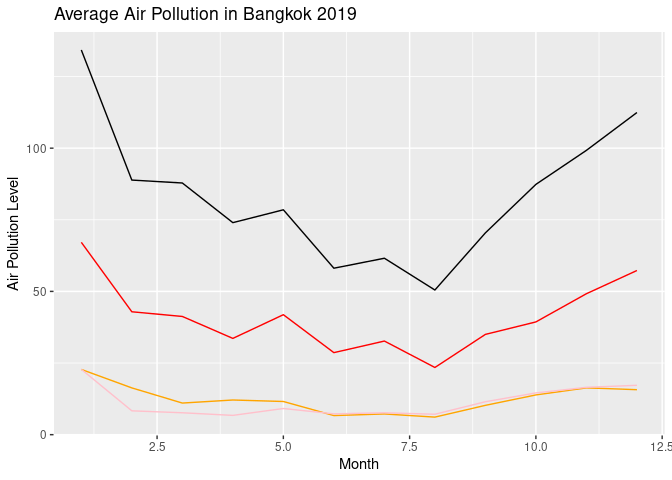
\includegraphics{Finalproject_files/figure-latex/unnamed-chunk-6-1.pdf}

As we can see from the graph, the local winter season (from October to
next year's February) has overall higher air pollution in all of the
four indexes. The reason is that when Bangkok is in winter, the air
temperature will be lower. The density of cold air is higher than that
of warm air, so cold air moves slower than warm air. Then the pollutants
in the air also move slower in winter because they tend to accumulate
and be trapped in the original area. Therefore, the air pollution in
winter will be higher than summer, which usually has warmer air. We can
also find that in Bangkok's rainy seasons, the air pollution level is
the lowest in a year. Besides the explanation from air density, I
believe the precipitation and humidity could also be the reasons. The
water can make the particulate matters accumulate and rush them to the
ground, which makes the air more clear. As we can see from the graph,
the PM2.5 and PM10 levels are decreased more than O3 and NO2. This is
because O3 and NO2 are actually toxic air, not particulate matters.
Therefore, they are hardly influenced in the rainy seasons. However,
interaction of NO2 and SO2 will bring acid rain, which harms sensitive
ecosystems in a large scale. We need to keep the toxic air in the least
possible level.

Now I come to the comparison of air quality between 2019 and 2020. For
the air pollution data of Bangkok in 2020, I first read the file and do
some basic data cleaning, including selecting ideal columns for analysis
and omitting NA values.

\begin{Shaded}
\begin{Highlighting}[]
\NormalTok{ap20\_raw }\OtherTok{\textless{}{-}} \FunctionTok{read.csv}\NormalTok{(}\StringTok{"bangkok{-}air20.csv"}\NormalTok{)}
\NormalTok{ap20\_new }\OtherTok{\textless{}{-}}\NormalTok{ dplyr}\SpecialCharTok{::}\FunctionTok{select}\NormalTok{(ap20\_raw, }\FunctionTok{c}\NormalTok{(}\SpecialCharTok{{-}}\NormalTok{so2,}\SpecialCharTok{{-}}\NormalTok{co))}
\NormalTok{ap20 }\OtherTok{\textless{}{-}} \FunctionTok{na.omit}\NormalTok{(ap20\_new)}
\FunctionTok{head}\NormalTok{(ap20)}
\end{Highlighting}
\end{Shaded}

\begin{verbatim}
##         date pm25 pm10 o3 no2
## 1 October-20   56   21  7  12
## 2 October-20   48   25 12  14
## 3 October-20   57   18 11  12
## 4 October-20   43   23 10   9
## 5 October-20   58   26 12  12
## 6 October-20   68   28 12   9
\end{verbatim}

Since we want to compare the overall air quality between 2019 and 2020
in Bangkok, we need to calculate the average level of each pollutants in
both years and make a comparison. I will make a table to directly
compare the pollution levels, and I expect the air quality in 2020 will
be better than the air quality in 2019. In the table, if the average
level of an air pollutant in 2020 is lower than 2019, it will have a
``TRUE'' answer.

\begin{Shaded}
\begin{Highlighting}[]
\NormalTok{pm25\_comparison }\OtherTok{\textless{}{-}} \FunctionTok{mean}\NormalTok{(ap20}\SpecialCharTok{$}\NormalTok{pm25) }\SpecialCharTok{\textless{}} \FunctionTok{mean}\NormalTok{(ap19}\SpecialCharTok{$}\NormalTok{pm25)}
\NormalTok{pm10\_comparison }\OtherTok{\textless{}{-}} \FunctionTok{mean}\NormalTok{(ap20}\SpecialCharTok{$}\NormalTok{pm10) }\SpecialCharTok{\textless{}} \FunctionTok{mean}\NormalTok{(ap19}\SpecialCharTok{$}\NormalTok{pm10)}
\NormalTok{o3\_comparison }\OtherTok{\textless{}{-}} \FunctionTok{mean}\NormalTok{(ap20}\SpecialCharTok{$}\NormalTok{o3) }\SpecialCharTok{\textless{}} \FunctionTok{mean}\NormalTok{(ap19}\SpecialCharTok{$}\NormalTok{o3)}
\NormalTok{no2\_comparison }\OtherTok{\textless{}{-}} \FunctionTok{mean}\NormalTok{(ap20}\SpecialCharTok{$}\NormalTok{no2) }\SpecialCharTok{\textless{}} \FunctionTok{mean}\NormalTok{(ap19}\SpecialCharTok{$}\NormalTok{no2)}
\NormalTok{comparison }\OtherTok{\textless{}{-}} \FunctionTok{data.frame}\NormalTok{(}
  \AttributeTok{AQ\_Index =} \FunctionTok{c}\NormalTok{(}\StringTok{"PM2.5"}\NormalTok{,}\StringTok{"PM10"}\NormalTok{,}\StringTok{"O3"}\NormalTok{,}\StringTok{"NO2"}\NormalTok{), }
  \AttributeTok{Result =} \FunctionTok{c}\NormalTok{(pm25\_comparison,pm10\_comparison,o3\_comparison,no2\_comparison))}
\NormalTok{comparison}
\end{Highlighting}
\end{Shaded}

\begin{verbatim}
##   AQ_Index Result
## 1    PM2.5   TRUE
## 2     PM10   TRUE
## 3       O3   TRUE
## 4      NO2   TRUE
\end{verbatim}

We can clearly see that, all of the pollutant levels in 2020 is lower
than 2019. It seems that under the COVID-19 pandemic, the air quality in
Bangkok became better. Possible reasons behind this phenomenon is that
under the COVID-19 quarantine requirements from the government, people
go out less and use less transportation. Therefore, the air quality is
better off.

For next part of analysis on the socio-economic factors behind the air
pollution in Bangkok, I decide to use the shapefiles data from Thailand
government. I will first download the data from the sources and store
them into my R ``work'' directory. The data I am going to download and
use are Bangkok's map and according population level (multipolygons),
the location of bikeways (multilinestrings), locations and quantities of
waste centers (points), and locations of gas stations (points).

\begin{Shaded}
\begin{Highlighting}[]
\FunctionTok{dir.create}\NormalTok{(}\StringTok{"../work/shapefiles"}\NormalTok{)}
\end{Highlighting}
\end{Shaded}

\begin{verbatim}
## Warning in dir.create("../work/shapefiles"): '../work/shapefiles' already exists
\end{verbatim}

\begin{Shaded}
\begin{Highlighting}[]
\FunctionTok{download.file}\NormalTok{(}\StringTok{"https://data.go.th/dataset/0199eb7f{-}6726{-}4947{-}8f98{-}e11652e82ae1/resource/090039e1{-}d33c{-}4341{-}a99a{-}cabe6916926d/download/waste\_center.zip"}\NormalTok{,}
              \StringTok{"../work/shapefiles/waste\_center.zip"}\NormalTok{)}
\FunctionTok{unzip}\NormalTok{(}\StringTok{"../work/shapefiles/waste\_center.zip"}\NormalTok{,}
      \AttributeTok{exdir=}\StringTok{"..work/shapefiles/bangkok\_waste"}\NormalTok{)}

\FunctionTok{download.file}\NormalTok{(}\StringTok{"https://data.go.th/dataset/04d564b5{-}b0db{-}48f9{-}ba41{-}b44b0422deec/resource/7c2c2c0b{-}1e7f{-}4437{-}b973{-}35308cb29f72/download/bike\_way.zip"}\NormalTok{,}
              \StringTok{"../work/shapefiles/bike\_way.zip"}\NormalTok{)}
\FunctionTok{unzip}\NormalTok{(}\StringTok{"../work/shapefiles/bike\_way.zip"}\NormalTok{,}
      \AttributeTok{exdir=}\StringTok{"..work/shapefiles/bikeway"}\NormalTok{)}

\FunctionTok{download.file}\NormalTok{(}\StringTok{"https://data.go.th/dataset/663ed528{-}97d7{-}4dd2{-}a463{-}be865e6fda28/resource/22667479{-}6786{-}495a{-}8606{-}c9b1dc433af2/download/district.zip"}\NormalTok{,}
              \StringTok{"../work/shapefiles/district.zip"}\NormalTok{)}
\FunctionTok{unzip}\NormalTok{(}\StringTok{"../work/shapefiles/district.zip"}\NormalTok{,}
      \AttributeTok{exdir=}\StringTok{"..work/shapefiles/ds"}\NormalTok{)}

\FunctionTok{download.file}\NormalTok{(}\StringTok{"https://data.go.th/dataset/9f8ed877{-}dfd8{-}43ec{-}b13d{-}33c05fb8ba2c/resource/90871776{-}e514{-}41c5{-}955a{-}8f258bd6f8ca/download/oil\_service.zip"}\NormalTok{,}
              \StringTok{"../work/shapefiles/oil\_service.zip"}\NormalTok{)}
\FunctionTok{unzip}\NormalTok{(}\StringTok{"../work/shapefiles/oil\_service.zip"}\NormalTok{,}
      \AttributeTok{exdir=}\StringTok{"..work/shapefiles/gas"}\NormalTok{)}
\end{Highlighting}
\end{Shaded}

After downloading the data, I can begin to read and plot the data. For
the second part of the below code chunk, I am trying to put the layers
of gas stations, bikeways, and waste centers above the layer of Bangkok
50 districts map. The white to brown color bar represents the number of
communities in each district of Bangkok, and it can show how many people
live in this district. So, if the area is red, then there lives more
residents then the white area. The gray circle represent the location of
waste centers in Bangkok, and their size represent the quantities of
waste centers in that district. The red points represent the gas
station, and one point represents one gas station. I also draw the major
bikeways in Bangkok, colored as green lines.

\begin{Shaded}
\begin{Highlighting}[]
\NormalTok{bangkok }\OtherTok{\textless{}{-}} \FunctionTok{st\_read}\NormalTok{(}\StringTok{"..work/shapefiles/ds/"}\NormalTok{)}
\end{Highlighting}
\end{Shaded}

\begin{verbatim}
## Reading layer `district' from data source 
##   `/home/jovyan/ESPM_157/FinalProject/work/..work/shapefiles/ds' 
##   using driver `ESRI Shapefile'
## Simple feature collection with 50 features and 14 fields
## Geometry type: POLYGON
## Dimension:     XY
## Bounding box:  xmin: 643535.3 ymin: 1492185 xmax: 709543.8 ymax: 1543272
## Projected CRS: WGS 84 / UTM zone 47N
\end{verbatim}

\begin{Shaded}
\begin{Highlighting}[]
\NormalTok{waste }\OtherTok{\textless{}{-}} \FunctionTok{st\_read}\NormalTok{(}\StringTok{"..work/shapefiles/bangkok\_waste/"}\NormalTok{)}
\end{Highlighting}
\end{Shaded}

\begin{verbatim}
## Warning in CPL_read_ogr(dsn, layer, query, as.character(options),
## quiet, : GDAL Error 4: Unable to open /home/jovyan/
## ESPM_157/FinalProject/work/..work/shapefiles/bangkok_waste/
## thiitangsuunykamcchadkhyaainekhtphuuenthiikrungethphmhaankhr.shx or /
## home/jovyan/ESPM_157/FinalProject/work/..work/shapefiles/bangkok_waste/
## thiitangsuunykamcchadkhyaainekhtphuuenthiikrungethphmhaankhr.SHX. Set
## SHAPE_RESTORE_SHX config option to YES to restore or create it.
\end{verbatim}

\begin{verbatim}
## Warning in CPL_read_ogr(dsn, layer, query, as.character(options),
## quiet, : GDAL Error 4: Failed to open file /home/jovyan/
## ESPM_157/FinalProject/work/..work/shapefiles/bangkok_waste/
## thiitangsuunykamcchadkhyaainekhtphuuenthiikrungethphmhaankhr.shp.It may be
## corrupt or read-only file accessed in update mode.
\end{verbatim}

\begin{verbatim}
## Reading layer `waste_center' from data source 
##   `/home/jovyan/ESPM_157/FinalProject/work/..work/shapefiles/bangkok_waste' 
##   using driver `ESRI Shapefile'
## Simple feature collection with 3 features and 5 fields
## Geometry type: POINT
## Dimension:     XY
## Bounding box:  xmin: 646416.1 ymin: 1516814 xmax: 681915.7 ymax: 1536384
## Projected CRS: WGS 84 / UTM zone 47N
\end{verbatim}

\begin{Shaded}
\begin{Highlighting}[]
\NormalTok{bw }\OtherTok{\textless{}{-}} \FunctionTok{st\_read}\NormalTok{(}\StringTok{"..work/shapefiles/bikeway/"}\NormalTok{)}
\end{Highlighting}
\end{Shaded}

\begin{verbatim}
## Reading layer `bike_way' from data source 
##   `/home/jovyan/ESPM_157/FinalProject/work/..work/shapefiles/bikeway' 
##   using driver `ESRI Shapefile'
## Simple feature collection with 31 features and 5 fields
## Geometry type: MULTILINESTRING
## Dimension:     XY
## Bounding box:  xmin: 643572.1 ymin: 1507251 xmax: 687719.9 ymax: 1541000
## Projected CRS: WGS 84 / UTM zone 47N
\end{verbatim}

\begin{Shaded}
\begin{Highlighting}[]
\NormalTok{gs }\OtherTok{\textless{}{-}} \FunctionTok{st\_read}\NormalTok{(}\StringTok{"..work/shapefiles/gas/"}\NormalTok{)}
\end{Highlighting}
\end{Shaded}

\begin{verbatim}
## Reading layer `oil_service' from data source 
##   `/home/jovyan/ESPM_157/FinalProject/work/..work/shapefiles/gas' 
##   using driver `ESRI Shapefile'
## Simple feature collection with 513 features and 6 fields
## Geometry type: POINT
## Dimension:     XY
## Bounding box:  xmin: -1.797693e+308 ymin: -1.797693e+308 xmax: 707603.9 ymax: 1542854
## Projected CRS: WGS 84 / UTM zone 47N
\end{verbatim}

\begin{Shaded}
\begin{Highlighting}[]
\FunctionTok{tm\_shape}\NormalTok{(bangkok) }\SpecialCharTok{+} \FunctionTok{tm\_polygons}\NormalTok{(}\AttributeTok{col =} \StringTok{"num\_comm"}\NormalTok{)}\SpecialCharTok{+}
  \FunctionTok{tm\_shape}\NormalTok{(waste) }\SpecialCharTok{+} \FunctionTok{tm\_bubbles}\NormalTok{(}\AttributeTok{size =} \StringTok{"quantity"}\NormalTok{, }\AttributeTok{scale =} \FloatTok{1.5}\NormalTok{) }\SpecialCharTok{+} \FunctionTok{tm\_text}\NormalTok{(}\StringTok{"quantity"}\NormalTok{, }\AttributeTok{just =} \StringTok{"left"}\NormalTok{, }\AttributeTok{xmod =} \FloatTok{0.5}\NormalTok{, }\AttributeTok{size =} \FloatTok{0.8}\NormalTok{) }\SpecialCharTok{+}
  \FunctionTok{tm\_shape}\NormalTok{(bw) }\SpecialCharTok{+} \FunctionTok{tm\_lines}\NormalTok{(}\AttributeTok{col =} \StringTok{"green"}\NormalTok{) }\SpecialCharTok{+} 
  \FunctionTok{tm\_shape}\NormalTok{(gs) }\SpecialCharTok{+} \FunctionTok{tm\_bubbles}\NormalTok{(}\AttributeTok{size=}\FloatTok{0.03}\NormalTok{, }\AttributeTok{col =} \StringTok{"red"}\NormalTok{) }\SpecialCharTok{+}
  \FunctionTok{tm\_legend}\NormalTok{(}\AttributeTok{outside =} \ConstantTok{TRUE}\NormalTok{)}
\end{Highlighting}
\end{Shaded}

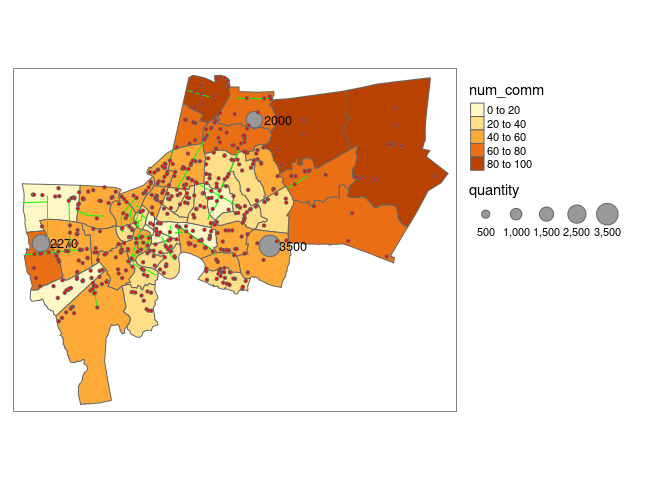
\includegraphics{Finalproject_files/figure-latex/unnamed-chunk-10-1.pdf}

As we can see from the image, the population is mostly in the right and
left districts of Bangkok. Something good from the image is that in the
right regions of Bangkok, which contain most of the population, we can
see very few gas stations. Gas stations typically bring NO2 and SO2 to
the atmosphere and harms the air quality. The small number of gas
stations in the right regions will not bring too many negative impacts
on the local air quality. Also, the waste centers are not in the right
regions. However, we can see that the most of waste centers are still in
the area which are highly populated (orange to red colors). This
phenomenon reminds me of the concept of environmental justice, which
means that some people, with lower education level, income level, worse
communities, etc., will typically experience more environmental
pollution than the people with high levels of income or education.
People who live in these districts are usually in bad
communities{[}1{]}, and they needed to suffer from the pollution to the
environment from these landfills. These areas are called the ``Desperate
Area'' in Bangkok, and we really need to make efforts to solve this
environmental injustice issue.

For the next part of analysis, I am going to research the natural factor
that influence the air quality in Bangkok. I decide to dive into two
factors, which are the geographical characteristics of Bangkok and
weather here. First, I download the geographical raster data from Open
Data Thailand.

\begin{Shaded}
\begin{Highlighting}[]
\FunctionTok{dir.create}\NormalTok{(}\StringTok{"../work/ls"}\NormalTok{)}
\end{Highlighting}
\end{Shaded}

\begin{verbatim}
## Warning in dir.create("../work/ls"): '../work/ls' already exists
\end{verbatim}

\begin{Shaded}
\begin{Highlighting}[]
\FunctionTok{download.file}\NormalTok{(}\StringTok{"http://www.savgis.org/Thailand/DEM/ThaiDEM500\_0000400000\_0011200000.zip"}\NormalTok{,}
              \StringTok{"../work/ls/ThaiDEM500\_0000400000\_0011200000.zip"}\NormalTok{)}
\FunctionTok{unzip}\NormalTok{(}\StringTok{"../work/ls/ThaiDEM500\_0000400000\_0011200000.zip"}\NormalTok{,}
      \AttributeTok{exdir=}\StringTok{"..work/ls/Thails"}\NormalTok{)}

\FunctionTok{download.file}\NormalTok{(}\StringTok{"http://www.savgis.org/Thailand/Rainfall.zip"}\NormalTok{,}
              \StringTok{"../work/shapefiles/Rainfall.zip"}\NormalTok{)}
\FunctionTok{unzip}\NormalTok{(}\StringTok{"../work/shapefiles/Rainfall.zip"}\NormalTok{,}
      \AttributeTok{exdir=}\StringTok{"..work/shapefiles/rainfall"}\NormalTok{)}
\end{Highlighting}
\end{Shaded}

After downloading the data, I can begin to plot the raster data by tmap
method. First I plot the basic elevation graph of central Thailand
region colored as ``heated map''. The green area will have low
elevation, namely the plain, and the red area will have high elevation,
namely the mountainous areas. Bangkok is on the olive green area with
very low elevation. There is also a color bar and quantile chart beside
the image. The quantile chart is used to represent the distribution of
elevations on this area.

\begin{Shaded}
\begin{Highlighting}[]
\NormalTok{area1 }\OtherTok{\textless{}{-}} \FunctionTok{raster}\NormalTok{(}\StringTok{"..work/ls/Thails/ThaiDEM500\_0000400000\_0011200000.asc"}\NormalTok{)}
\FunctionTok{tm\_shape}\NormalTok{(area1) }\SpecialCharTok{+}
  \FunctionTok{tm\_raster}\NormalTok{(}\AttributeTok{style =} \StringTok{"quantile"}\NormalTok{, }\AttributeTok{n =} \DecValTok{10}\NormalTok{, }\AttributeTok{title =} \StringTok{"Elevation (m)"}\NormalTok{,}
            \AttributeTok{palette =} \FunctionTok{colorRampPalette}\NormalTok{( }\FunctionTok{c}\NormalTok{(}\StringTok{"darkolivegreen4"}\NormalTok{,}\StringTok{"yellow"}\NormalTok{, }\StringTok{"brown"}\NormalTok{))(}\DecValTok{10}\NormalTok{),}
            \AttributeTok{legend.hist =} \ConstantTok{TRUE}\NormalTok{)}\SpecialCharTok{+}
  \FunctionTok{tm\_legend}\NormalTok{(}\AttributeTok{outside =} \ConstantTok{TRUE}\NormalTok{, }\AttributeTok{hist.width =} \DecValTok{5}\NormalTok{)}
\end{Highlighting}
\end{Shaded}

\begin{verbatim}
## Warning: The projection of the shape object area1 is not known, while it seems
## to be projected.
\end{verbatim}

\begin{verbatim}
## Warning: Current projection of shape area1 unknown and cannot be determined.
\end{verbatim}

\begin{verbatim}
## Variable(s) "NA" contains positive and negative values, so midpoint is set to 0. Set midpoint = NA to show the full spectrum of the color palette.
\end{verbatim}

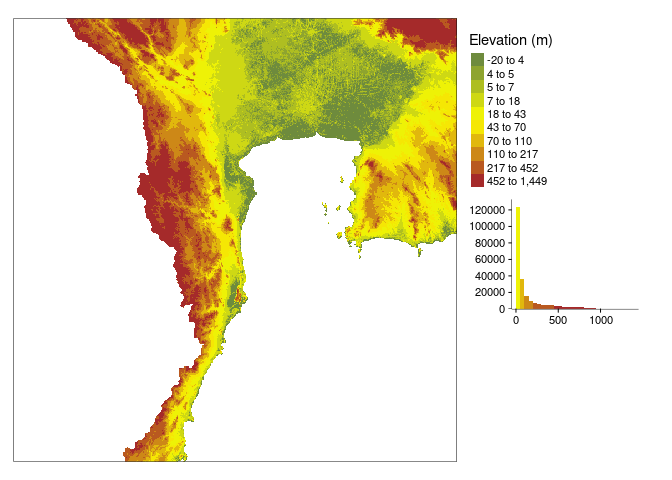
\includegraphics{Finalproject_files/figure-latex/unnamed-chunk-12-1.pdf}

As we can see from the graph, Bangkok is surrounded by the mountainous
areas in the central part of Thailand. This difference of elevations
creates a basin area which actually makes the air pollutants above
Bangkok hard to spread to other regions because the mountains will block
the wind. This geography characteristic may continue to worsen the air
quality in Bangkok by accumulating the air pollutants and holding them
from spreading to other places. Therefore, geography is a potential
factor to influence the local air quality in Bangkok.

Besides the geography, I am going to research the relationship between
local weather and air quality. At the beginning, I need to use my API
key to call Bangkok weather data from Open Weather Map. The city ID of
Bangkok is 1609348, and I choose to extract the monthly aggregated data
for year 2020 from this platform. After extracting them, I prepare them
to the JSON format for further analysis. I store the raw JSON data into
m1, m2, m3, etc. which means month 1, month 2, month 3, etc. to make
tables.

\begin{Shaded}
\begin{Highlighting}[]
\NormalTok{dm1 }\OtherTok{\textless{}{-}} \FunctionTok{GET}\NormalTok{(}\StringTok{"history.openweathermap.org/data/2.5/aggregated/month?id=1609348\&month=1\&appid=e969380692a03d6dee11c0a5cf7bc5e3"}\NormalTok{)}
\NormalTok{m1 }\OtherTok{\textless{}{-}} \FunctionTok{fromJSON}\NormalTok{(}\FunctionTok{rawToChar}\NormalTok{(dm1}\SpecialCharTok{$}\NormalTok{content))}
\NormalTok{dm2 }\OtherTok{\textless{}{-}} \FunctionTok{GET}\NormalTok{(}\StringTok{"history.openweathermap.org/data/2.5/aggregated/month?id=1609348\&month=2\&appid=e969380692a03d6dee11c0a5cf7bc5e3"}\NormalTok{)}
\NormalTok{m2 }\OtherTok{\textless{}{-}} \FunctionTok{fromJSON}\NormalTok{(}\FunctionTok{rawToChar}\NormalTok{(dm2}\SpecialCharTok{$}\NormalTok{content))}
\NormalTok{dm3 }\OtherTok{\textless{}{-}} \FunctionTok{GET}\NormalTok{(}\StringTok{"history.openweathermap.org/data/2.5/aggregated/month?id=1609348\&month=3\&appid=e969380692a03d6dee11c0a5cf7bc5e3"}\NormalTok{)}
\NormalTok{m3 }\OtherTok{\textless{}{-}} \FunctionTok{fromJSON}\NormalTok{(}\FunctionTok{rawToChar}\NormalTok{(dm3}\SpecialCharTok{$}\NormalTok{content))}
\NormalTok{dm4 }\OtherTok{\textless{}{-}} \FunctionTok{GET}\NormalTok{(}\StringTok{"history.openweathermap.org/data/2.5/aggregated/month?id=1609348\&month=4\&appid=e969380692a03d6dee11c0a5cf7bc5e3"}\NormalTok{)}
\NormalTok{m4 }\OtherTok{\textless{}{-}} \FunctionTok{fromJSON}\NormalTok{(}\FunctionTok{rawToChar}\NormalTok{(dm4}\SpecialCharTok{$}\NormalTok{content))}
\NormalTok{dm5 }\OtherTok{\textless{}{-}} \FunctionTok{GET}\NormalTok{(}\StringTok{"history.openweathermap.org/data/2.5/aggregated/month?id=1609348\&month=5\&appid=e969380692a03d6dee11c0a5cf7bc5e3"}\NormalTok{)}
\NormalTok{m5 }\OtherTok{\textless{}{-}} \FunctionTok{fromJSON}\NormalTok{(}\FunctionTok{rawToChar}\NormalTok{(dm5}\SpecialCharTok{$}\NormalTok{content))}
\NormalTok{dm6 }\OtherTok{\textless{}{-}} \FunctionTok{GET}\NormalTok{(}\StringTok{"history.openweathermap.org/data/2.5/aggregated/month?id=1609348\&month=6\&appid=e969380692a03d6dee11c0a5cf7bc5e3"}\NormalTok{)}
\NormalTok{m6 }\OtherTok{\textless{}{-}} \FunctionTok{fromJSON}\NormalTok{(}\FunctionTok{rawToChar}\NormalTok{(dm6}\SpecialCharTok{$}\NormalTok{content))}
\NormalTok{dm7 }\OtherTok{\textless{}{-}} \FunctionTok{GET}\NormalTok{(}\StringTok{"history.openweathermap.org/data/2.5/aggregated/month?id=1609348\&month=7\&appid=e969380692a03d6dee11c0a5cf7bc5e3"}\NormalTok{)}
\NormalTok{m7 }\OtherTok{\textless{}{-}} \FunctionTok{fromJSON}\NormalTok{(}\FunctionTok{rawToChar}\NormalTok{(dm7}\SpecialCharTok{$}\NormalTok{content))}
\NormalTok{dm8 }\OtherTok{\textless{}{-}} \FunctionTok{GET}\NormalTok{(}\StringTok{"history.openweathermap.org/data/2.5/aggregated/month?id=1609348\&month=8\&appid=e969380692a03d6dee11c0a5cf7bc5e3"}\NormalTok{)}
\NormalTok{m8 }\OtherTok{\textless{}{-}} \FunctionTok{fromJSON}\NormalTok{(}\FunctionTok{rawToChar}\NormalTok{(dm8}\SpecialCharTok{$}\NormalTok{content))}
\NormalTok{dm9 }\OtherTok{\textless{}{-}} \FunctionTok{GET}\NormalTok{(}\StringTok{"history.openweathermap.org/data/2.5/aggregated/month?id=1609348\&month=9\&appid=e969380692a03d6dee11c0a5cf7bc5e3"}\NormalTok{)}
\NormalTok{m9 }\OtherTok{\textless{}{-}} \FunctionTok{fromJSON}\NormalTok{(}\FunctionTok{rawToChar}\NormalTok{(dm9}\SpecialCharTok{$}\NormalTok{content))}
\NormalTok{dm10 }\OtherTok{\textless{}{-}} \FunctionTok{GET}\NormalTok{(}\StringTok{"history.openweathermap.org/data/2.5/aggregated/month?id=1609348\&month=10\&appid=e969380692a03d6dee11c0a5cf7bc5e3"}\NormalTok{)}
\NormalTok{m10 }\OtherTok{\textless{}{-}} \FunctionTok{fromJSON}\NormalTok{(}\FunctionTok{rawToChar}\NormalTok{(dm10}\SpecialCharTok{$}\NormalTok{content))}
\NormalTok{dm11 }\OtherTok{\textless{}{-}} \FunctionTok{GET}\NormalTok{(}\StringTok{"history.openweathermap.org/data/2.5/aggregated/month?id=1609348\&month=11\&appid=e969380692a03d6dee11c0a5cf7bc5e3"}\NormalTok{)}
\NormalTok{m11 }\OtherTok{\textless{}{-}} \FunctionTok{fromJSON}\NormalTok{(}\FunctionTok{rawToChar}\NormalTok{(dm11}\SpecialCharTok{$}\NormalTok{content))}
\NormalTok{dm12 }\OtherTok{\textless{}{-}} \FunctionTok{GET}\NormalTok{(}\StringTok{"history.openweathermap.org/data/2.5/aggregated/month?id=1609348\&month=12\&appid=e969380692a03d6dee11c0a5cf7bc5e3"}\NormalTok{)}
\NormalTok{m12 }\OtherTok{\textless{}{-}} \FunctionTok{fromJSON}\NormalTok{(}\FunctionTok{rawToChar}\NormalTok{(dm12}\SpecialCharTok{$}\NormalTok{content))}
\end{Highlighting}
\end{Shaded}

Below, I am trying to create a table to show the average humidity,
average wind speed, and average precipitation by twelve months in 2020.
This table will be convenient when merging with the table of air
pollution data before.

\begin{Shaded}
\begin{Highlighting}[]
\NormalTok{month }\OtherTok{\textless{}{-}} \FunctionTok{c}\NormalTok{(}\DecValTok{1}\NormalTok{,}\DecValTok{2}\NormalTok{,}\DecValTok{3}\NormalTok{,}\DecValTok{4}\NormalTok{,}\DecValTok{5}\NormalTok{,}\DecValTok{6}\NormalTok{,}\DecValTok{7}\NormalTok{,}\DecValTok{8}\NormalTok{,}\DecValTok{9}\NormalTok{,}\DecValTok{10}\NormalTok{,}\DecValTok{11}\NormalTok{,}\DecValTok{12}\NormalTok{)}
\NormalTok{mean\_humidity }\OtherTok{\textless{}{-}} \FunctionTok{c}\NormalTok{(m1[[}\StringTok{"result"}\NormalTok{]][[}\StringTok{"humidity"}\NormalTok{]][[}\StringTok{"mean"}\NormalTok{]],m2[[}\StringTok{"result"}\NormalTok{]][[}\StringTok{"humidity"}\NormalTok{]][[}\StringTok{"mean"}\NormalTok{]],m3[[}\StringTok{"result"}\NormalTok{]][[}\StringTok{"humidity"}\NormalTok{]][[}\StringTok{"mean"}\NormalTok{]],m4[[}\StringTok{"result"}\NormalTok{]][[}\StringTok{"humidity"}\NormalTok{]][[}\StringTok{"mean"}\NormalTok{]],}
\NormalTok{                   m5[[}\StringTok{"result"}\NormalTok{]][[}\StringTok{"humidity"}\NormalTok{]][[}\StringTok{"mean"}\NormalTok{]],m6[[}\StringTok{"result"}\NormalTok{]][[}\StringTok{"humidity"}\NormalTok{]][[}\StringTok{"mean"}\NormalTok{]],m7[[}\StringTok{"result"}\NormalTok{]][[}\StringTok{"humidity"}\NormalTok{]][[}\StringTok{"mean"}\NormalTok{]],m8[[}\StringTok{"result"}\NormalTok{]][[}\StringTok{"humidity"}\NormalTok{]][[}\StringTok{"mean"}\NormalTok{]],}
\NormalTok{                   m9[[}\StringTok{"result"}\NormalTok{]][[}\StringTok{"humidity"}\NormalTok{]][[}\StringTok{"mean"}\NormalTok{]],m10[[}\StringTok{"result"}\NormalTok{]][[}\StringTok{"humidity"}\NormalTok{]][[}\StringTok{"mean"}\NormalTok{]],m11[[}\StringTok{"result"}\NormalTok{]][[}\StringTok{"humidity"}\NormalTok{]][[}\StringTok{"mean"}\NormalTok{]],m12[[}\StringTok{"result"}\NormalTok{]][[}\StringTok{"humidity"}\NormalTok{]][[}\StringTok{"mean"}\NormalTok{]])}
\NormalTok{mean\_windspeed }\OtherTok{\textless{}{-}} \FunctionTok{c}\NormalTok{(m1[[}\StringTok{"result"}\NormalTok{]][[}\StringTok{"wind"}\NormalTok{]][[}\StringTok{"mean"}\NormalTok{]],m2[[}\StringTok{"result"}\NormalTok{]][[}\StringTok{"wind"}\NormalTok{]][[}\StringTok{"mean"}\NormalTok{]],m3[[}\StringTok{"result"}\NormalTok{]][[}\StringTok{"wind"}\NormalTok{]][[}\StringTok{"mean"}\NormalTok{]],m4[[}\StringTok{"result"}\NormalTok{]][[}\StringTok{"wind"}\NormalTok{]][[}\StringTok{"mean"}\NormalTok{]],}
\NormalTok{                   m5[[}\StringTok{"result"}\NormalTok{]][[}\StringTok{"wind"}\NormalTok{]][[}\StringTok{"mean"}\NormalTok{]],m6[[}\StringTok{"result"}\NormalTok{]][[}\StringTok{"wind"}\NormalTok{]][[}\StringTok{"mean"}\NormalTok{]],m7[[}\StringTok{"result"}\NormalTok{]][[}\StringTok{"wind"}\NormalTok{]][[}\StringTok{"mean"}\NormalTok{]],m8[[}\StringTok{"result"}\NormalTok{]][[}\StringTok{"wind"}\NormalTok{]][[}\StringTok{"mean"}\NormalTok{]],}
\NormalTok{                   m9[[}\StringTok{"result"}\NormalTok{]][[}\StringTok{"wind"}\NormalTok{]][[}\StringTok{"mean"}\NormalTok{]],m10[[}\StringTok{"result"}\NormalTok{]][[}\StringTok{"wind"}\NormalTok{]][[}\StringTok{"mean"}\NormalTok{]],m11[[}\StringTok{"result"}\NormalTok{]][[}\StringTok{"wind"}\NormalTok{]][[}\StringTok{"mean"}\NormalTok{]],m12[[}\StringTok{"result"}\NormalTok{]][[}\StringTok{"wind"}\NormalTok{]][[}\StringTok{"mean"}\NormalTok{]])}
\NormalTok{mean\_precipitation }\OtherTok{\textless{}{-}} \FunctionTok{c}\NormalTok{(m1[[}\StringTok{"result"}\NormalTok{]][[}\StringTok{"precipitation"}\NormalTok{]][[}\StringTok{"mean"}\NormalTok{]],m2[[}\StringTok{"result"}\NormalTok{]][[}\StringTok{"precipitation"}\NormalTok{]][[}\StringTok{"mean"}\NormalTok{]],m3[[}\StringTok{"result"}\NormalTok{]][[}\StringTok{"precipitation"}\NormalTok{]][[}\StringTok{"mean"}\NormalTok{]],m4[[}\StringTok{"result"}\NormalTok{]][[}\StringTok{"precipitation"}\NormalTok{]][[}\StringTok{"mean"}\NormalTok{]],}
\NormalTok{                   m5[[}\StringTok{"result"}\NormalTok{]][[}\StringTok{"precipitation"}\NormalTok{]][[}\StringTok{"mean"}\NormalTok{]],m6[[}\StringTok{"result"}\NormalTok{]][[}\StringTok{"precipitation"}\NormalTok{]][[}\StringTok{"mean"}\NormalTok{]],m7[[}\StringTok{"result"}\NormalTok{]][[}\StringTok{"precipitation"}\NormalTok{]][[}\StringTok{"mean"}\NormalTok{]],m8[[}\StringTok{"result"}\NormalTok{]][[}\StringTok{"precipitation"}\NormalTok{]][[}\StringTok{"mean"}\NormalTok{]],}
\NormalTok{                   m9[[}\StringTok{"result"}\NormalTok{]][[}\StringTok{"precipitation"}\NormalTok{]][[}\StringTok{"mean"}\NormalTok{]],m10[[}\StringTok{"result"}\NormalTok{]][[}\StringTok{"precipitation"}\NormalTok{]][[}\StringTok{"mean"}\NormalTok{]],m11[[}\StringTok{"result"}\NormalTok{]][[}\StringTok{"precipitation"}\NormalTok{]][[}\StringTok{"mean"}\NormalTok{]],m12[[}\StringTok{"result"}\NormalTok{]][[}\StringTok{"precipitation"}\NormalTok{]][[}\StringTok{"mean"}\NormalTok{]])}
\NormalTok{weather\_data2020 }\OtherTok{\textless{}{-}} \FunctionTok{data.frame}\NormalTok{(month,mean\_humidity,mean\_windspeed,mean\_precipitation)}
\NormalTok{weather\_data2020}
\end{Highlighting}
\end{Shaded}

\begin{verbatim}
##    month mean_humidity mean_windspeed mean_precipitation
## 1      1         63.79           2.69               0.04
## 2      2         63.88           3.07               0.04
## 3      3         68.26           3.77               0.08
## 4      4         68.24           3.56               0.07
## 5      5         69.42           3.33               0.09
## 6      6         72.73           3.33               0.18
## 7      7         72.55           3.45               0.10
## 8      8         73.70           3.38               0.13
## 9      9         78.25           2.85               0.20
## 10    10         79.40           2.43               0.22
## 11    11         69.33           2.69               0.09
## 12    12         62.42           2.80               0.03
\end{verbatim}

As I just prepared the data for air pollution in 2019, I need to make
some quick and basic data cleaning for the 2020 air quality dataset,
including grouping, calculating the average pollution level in each
month, and rearranging the dataset.

\begin{Shaded}
\begin{Highlighting}[]
\NormalTok{ap20sum }\OtherTok{\textless{}{-}}\NormalTok{ ap20 }\SpecialCharTok{\%\textgreater{}\%}
  \FunctionTok{group\_by}\NormalTok{(date) }\SpecialCharTok{\%\textgreater{}\%}
  \FunctionTok{summarise}\NormalTok{(}\AttributeTok{mean\_pm25 =} \FunctionTok{mean}\NormalTok{(pm25),}\AttributeTok{mean\_pm10 =} \FunctionTok{mean}\NormalTok{(pm10),}\AttributeTok{mean\_o3 =} \FunctionTok{mean}\NormalTok{(o3),}\AttributeTok{mean\_no2 =} \FunctionTok{mean}\NormalTok{(no2))}

\NormalTok{month20 }\OtherTok{\textless{}{-}} \FunctionTok{c}\NormalTok{(}\DecValTok{4}\NormalTok{,}\DecValTok{8}\NormalTok{,}\DecValTok{12}\NormalTok{,}\DecValTok{2}\NormalTok{,}\DecValTok{1}\NormalTok{,}\DecValTok{7}\NormalTok{,}\DecValTok{6}\NormalTok{,}\DecValTok{3}\NormalTok{,}\DecValTok{5}\NormalTok{,}\DecValTok{11}\NormalTok{,}\DecValTok{10}\NormalTok{,}\DecValTok{9}\NormalTok{)}
\NormalTok{itm20 }\OtherTok{\textless{}{-}}\NormalTok{ ap20sum }\SpecialCharTok{\%\textgreater{}\%} \FunctionTok{add\_column}\NormalTok{(}\AttributeTok{month =}\NormalTok{ month20)}
\NormalTok{ro\_ap20sum }\OtherTok{\textless{}{-}} \FunctionTok{arrange}\NormalTok{(dplyr}\SpecialCharTok{::}\FunctionTok{select}\NormalTok{(itm20[, }\FunctionTok{c}\NormalTok{(}\DecValTok{6}\NormalTok{,}\DecValTok{1}\NormalTok{,}\DecValTok{2}\NormalTok{,}\DecValTok{3}\NormalTok{,}\DecValTok{4}\NormalTok{,}\DecValTok{5}\NormalTok{)],}\SpecialCharTok{{-}}\NormalTok{date), month20)}
\end{Highlighting}
\end{Shaded}

After cleaning the data, I can merge the weather data in 2020 with the
air pollution 2020 data together, and I get the ``summary'' table. It
will be convenient for correlation analysis.

\begin{Shaded}
\begin{Highlighting}[]
\NormalTok{summary }\OtherTok{\textless{}{-}} \FunctionTok{merge}\NormalTok{(}\AttributeTok{x =}\NormalTok{ ro\_ap20sum, }\AttributeTok{y =}\NormalTok{ weather\_data2020, }\AttributeTok{by=}\StringTok{"month"}\NormalTok{,}\AttributeTok{all=}\ConstantTok{TRUE}\NormalTok{)}
\NormalTok{summary}
\end{Highlighting}
\end{Shaded}

\begin{verbatim}
##    month mean_pm25 mean_pm10   mean_o3  mean_no2 mean_humidity mean_windspeed
## 1      1 120.73333  60.13333 13.966667 14.833333         63.79           2.69
## 2      2 126.68966  64.79310 16.827586 11.965517         63.88           3.07
## 3      3  79.00000  37.89655 10.000000  5.931034         68.26           3.77
## 4      4  73.13793  33.41379 13.344828  5.517241         68.24           3.56
## 5      5  61.70968  27.67742 10.741935  4.161290         69.42           3.33
## 6      6  48.93333  21.30000  9.433333  5.933333         72.73           3.33
## 7      7  52.09677  23.22581 10.580645  6.645161         72.55           3.45
## 8      8  53.41935  25.32258  7.225806  5.870968         73.70           3.38
## 9      9  51.20000  24.83333  8.666667  6.833333         78.25           2.85
## 10    10  68.12903  32.70968  9.677419 13.645161         79.40           2.43
## 11    11  87.86667  43.86667 17.333333 15.066667         69.33           2.69
## 12    12 104.12903  52.48387 18.161290 18.709677         62.42           2.80
##    mean_precipitation
## 1                0.04
## 2                0.04
## 3                0.08
## 4                0.07
## 5                0.09
## 6                0.18
## 7                0.10
## 8                0.13
## 9                0.20
## 10               0.22
## 11               0.09
## 12               0.03
\end{verbatim}

Below, I am trying to create three graphs which explore the
relationships between different weather conditions (humidity, wind
speed, and precipitation) and air pollutants. They will be dot plots.
The x axis will be a certain weather condition, and the y axis will be
the pollution level for these four air pollutants. In each graph, the
cadet blue dots will be average PM2.5; the violet dots will be average
PM10, the green yellow dots will be average O3, and the black dots will
be average NO2.

\begin{Shaded}
\begin{Highlighting}[]
\FunctionTok{par}\NormalTok{(}\AttributeTok{mfrow =} \FunctionTok{c}\NormalTok{(}\DecValTok{2}\NormalTok{,}\DecValTok{2}\NormalTok{))}

\FunctionTok{plot}\NormalTok{(summary}\SpecialCharTok{$}\NormalTok{mean\_humidity,summary}\SpecialCharTok{$}\NormalTok{mean\_pm25,}\AttributeTok{col =} \StringTok{"cadetblue"}\NormalTok{,}\AttributeTok{xlab=}\StringTok{"Mean Humidity (\%)"}\NormalTok{, }\AttributeTok{ylab=}\StringTok{"Air Pollution level (ug/m3)"}\NormalTok{,}\AttributeTok{ylim=}\FunctionTok{c}\NormalTok{(}\DecValTok{0}\NormalTok{,}\DecValTok{130}\NormalTok{), }\AttributeTok{pch=}\StringTok{"●"}\NormalTok{,}\AttributeTok{cex.lab=}\FloatTok{0.8}\NormalTok{)}
\end{Highlighting}
\end{Shaded}

\begin{verbatim}
## Warning in plot.xy(xy, type, ...): conversion failure on '●' in 'mbcsToSbcs':
## dot substituted for <e2>
\end{verbatim}

\begin{verbatim}
## Warning in plot.xy(xy, type, ...): conversion failure on '●' in 'mbcsToSbcs':
## dot substituted for <97>
\end{verbatim}

\begin{verbatim}
## Warning in plot.xy(xy, type, ...): conversion failure on '●' in 'mbcsToSbcs':
## dot substituted for <8f>
\end{verbatim}

\begin{verbatim}
## Warning in plot.xy(xy, type, ...): font metrics unknown for Unicode character
## U+25cf
\end{verbatim}

\begin{verbatim}
## Warning in plot.xy(xy, type, ...): conversion failure on '●' in 'mbcsToSbcs':
## dot substituted for <e2>
\end{verbatim}

\begin{verbatim}
## Warning in plot.xy(xy, type, ...): conversion failure on '●' in 'mbcsToSbcs':
## dot substituted for <97>
\end{verbatim}

\begin{verbatim}
## Warning in plot.xy(xy, type, ...): conversion failure on '●' in 'mbcsToSbcs':
## dot substituted for <8f>
\end{verbatim}

\begin{verbatim}
## Warning in plot.xy(xy, type, ...): font metrics unknown for Unicode character
## U+25cf
\end{verbatim}

\begin{verbatim}
## Warning in plot.xy(xy, type, ...): conversion failure on '●' in 'mbcsToSbcs':
## dot substituted for <e2>
\end{verbatim}

\begin{verbatim}
## Warning in plot.xy(xy, type, ...): conversion failure on '●' in 'mbcsToSbcs':
## dot substituted for <97>
\end{verbatim}

\begin{verbatim}
## Warning in plot.xy(xy, type, ...): conversion failure on '●' in 'mbcsToSbcs':
## dot substituted for <8f>
\end{verbatim}

\begin{verbatim}
## Warning in plot.xy(xy, type, ...): font metrics unknown for Unicode character
## U+25cf
\end{verbatim}

\begin{verbatim}
## Warning in plot.xy(xy, type, ...): conversion failure on '●' in 'mbcsToSbcs':
## dot substituted for <e2>
\end{verbatim}

\begin{verbatim}
## Warning in plot.xy(xy, type, ...): conversion failure on '●' in 'mbcsToSbcs':
## dot substituted for <97>
\end{verbatim}

\begin{verbatim}
## Warning in plot.xy(xy, type, ...): conversion failure on '●' in 'mbcsToSbcs':
## dot substituted for <8f>
\end{verbatim}

\begin{verbatim}
## Warning in plot.xy(xy, type, ...): font metrics unknown for Unicode character
## U+25cf
\end{verbatim}

\begin{verbatim}
## Warning in plot.xy(xy, type, ...): conversion failure on '●' in 'mbcsToSbcs':
## dot substituted for <e2>
\end{verbatim}

\begin{verbatim}
## Warning in plot.xy(xy, type, ...): conversion failure on '●' in 'mbcsToSbcs':
## dot substituted for <97>
\end{verbatim}

\begin{verbatim}
## Warning in plot.xy(xy, type, ...): conversion failure on '●' in 'mbcsToSbcs':
## dot substituted for <8f>
\end{verbatim}

\begin{verbatim}
## Warning in plot.xy(xy, type, ...): font metrics unknown for Unicode character
## U+25cf
\end{verbatim}

\begin{verbatim}
## Warning in plot.xy(xy, type, ...): conversion failure on '●' in 'mbcsToSbcs':
## dot substituted for <e2>
\end{verbatim}

\begin{verbatim}
## Warning in plot.xy(xy, type, ...): conversion failure on '●' in 'mbcsToSbcs':
## dot substituted for <97>
\end{verbatim}

\begin{verbatim}
## Warning in plot.xy(xy, type, ...): conversion failure on '●' in 'mbcsToSbcs':
## dot substituted for <8f>
\end{verbatim}

\begin{verbatim}
## Warning in plot.xy(xy, type, ...): font metrics unknown for Unicode character
## U+25cf
\end{verbatim}

\begin{verbatim}
## Warning in plot.xy(xy, type, ...): conversion failure on '●' in 'mbcsToSbcs':
## dot substituted for <e2>
\end{verbatim}

\begin{verbatim}
## Warning in plot.xy(xy, type, ...): conversion failure on '●' in 'mbcsToSbcs':
## dot substituted for <97>
\end{verbatim}

\begin{verbatim}
## Warning in plot.xy(xy, type, ...): conversion failure on '●' in 'mbcsToSbcs':
## dot substituted for <8f>
\end{verbatim}

\begin{verbatim}
## Warning in plot.xy(xy, type, ...): font metrics unknown for Unicode character
## U+25cf
\end{verbatim}

\begin{verbatim}
## Warning in plot.xy(xy, type, ...): conversion failure on '●' in 'mbcsToSbcs':
## dot substituted for <e2>
\end{verbatim}

\begin{verbatim}
## Warning in plot.xy(xy, type, ...): conversion failure on '●' in 'mbcsToSbcs':
## dot substituted for <97>
\end{verbatim}

\begin{verbatim}
## Warning in plot.xy(xy, type, ...): conversion failure on '●' in 'mbcsToSbcs':
## dot substituted for <8f>
\end{verbatim}

\begin{verbatim}
## Warning in plot.xy(xy, type, ...): font metrics unknown for Unicode character
## U+25cf
\end{verbatim}

\begin{verbatim}
## Warning in plot.xy(xy, type, ...): conversion failure on '●' in 'mbcsToSbcs':
## dot substituted for <e2>
\end{verbatim}

\begin{verbatim}
## Warning in plot.xy(xy, type, ...): conversion failure on '●' in 'mbcsToSbcs':
## dot substituted for <97>
\end{verbatim}

\begin{verbatim}
## Warning in plot.xy(xy, type, ...): conversion failure on '●' in 'mbcsToSbcs':
## dot substituted for <8f>
\end{verbatim}

\begin{verbatim}
## Warning in plot.xy(xy, type, ...): font metrics unknown for Unicode character
## U+25cf
\end{verbatim}

\begin{verbatim}
## Warning in plot.xy(xy, type, ...): conversion failure on '●' in 'mbcsToSbcs':
## dot substituted for <e2>
\end{verbatim}

\begin{verbatim}
## Warning in plot.xy(xy, type, ...): conversion failure on '●' in 'mbcsToSbcs':
## dot substituted for <97>
\end{verbatim}

\begin{verbatim}
## Warning in plot.xy(xy, type, ...): conversion failure on '●' in 'mbcsToSbcs':
## dot substituted for <8f>
\end{verbatim}

\begin{verbatim}
## Warning in plot.xy(xy, type, ...): font metrics unknown for Unicode character
## U+25cf
\end{verbatim}

\begin{verbatim}
## Warning in plot.xy(xy, type, ...): conversion failure on '●' in 'mbcsToSbcs':
## dot substituted for <e2>
\end{verbatim}

\begin{verbatim}
## Warning in plot.xy(xy, type, ...): conversion failure on '●' in 'mbcsToSbcs':
## dot substituted for <97>
\end{verbatim}

\begin{verbatim}
## Warning in plot.xy(xy, type, ...): conversion failure on '●' in 'mbcsToSbcs':
## dot substituted for <8f>
\end{verbatim}

\begin{verbatim}
## Warning in plot.xy(xy, type, ...): font metrics unknown for Unicode character
## U+25cf
\end{verbatim}

\begin{verbatim}
## Warning in plot.xy(xy, type, ...): conversion failure on '●' in 'mbcsToSbcs':
## dot substituted for <e2>
\end{verbatim}

\begin{verbatim}
## Warning in plot.xy(xy, type, ...): conversion failure on '●' in 'mbcsToSbcs':
## dot substituted for <97>
\end{verbatim}

\begin{verbatim}
## Warning in plot.xy(xy, type, ...): conversion failure on '●' in 'mbcsToSbcs':
## dot substituted for <8f>
\end{verbatim}

\begin{verbatim}
## Warning in plot.xy(xy, type, ...): font metrics unknown for Unicode character
## U+25cf
\end{verbatim}

\begin{Shaded}
\begin{Highlighting}[]
\FunctionTok{points}\NormalTok{(summary}\SpecialCharTok{$}\NormalTok{mean\_humidity, summary}\SpecialCharTok{$}\NormalTok{mean\_pm10, }\AttributeTok{col=}\StringTok{"violetred4"}\NormalTok{,}\AttributeTok{pch=}\StringTok{"●"}\NormalTok{)}
\end{Highlighting}
\end{Shaded}

\begin{verbatim}
## Warning in plot.xy(xy.coords(x, y), type = type, ...): conversion failure on
## '●' in 'mbcsToSbcs': dot substituted for <e2>
\end{verbatim}

\begin{verbatim}
## Warning in plot.xy(xy.coords(x, y), type = type, ...): conversion failure on
## '●' in 'mbcsToSbcs': dot substituted for <97>
\end{verbatim}

\begin{verbatim}
## Warning in plot.xy(xy.coords(x, y), type = type, ...): conversion failure on
## '●' in 'mbcsToSbcs': dot substituted for <8f>
\end{verbatim}

\begin{verbatim}
## Warning in plot.xy(xy.coords(x, y), type = type, ...): font metrics unknown for
## Unicode character U+25cf
\end{verbatim}

\begin{verbatim}
## Warning in plot.xy(xy.coords(x, y), type = type, ...): conversion failure on
## '●' in 'mbcsToSbcs': dot substituted for <e2>
\end{verbatim}

\begin{verbatim}
## Warning in plot.xy(xy.coords(x, y), type = type, ...): conversion failure on
## '●' in 'mbcsToSbcs': dot substituted for <97>
\end{verbatim}

\begin{verbatim}
## Warning in plot.xy(xy.coords(x, y), type = type, ...): conversion failure on
## '●' in 'mbcsToSbcs': dot substituted for <8f>
\end{verbatim}

\begin{verbatim}
## Warning in plot.xy(xy.coords(x, y), type = type, ...): font metrics unknown for
## Unicode character U+25cf
\end{verbatim}

\begin{verbatim}
## Warning in plot.xy(xy.coords(x, y), type = type, ...): conversion failure on
## '●' in 'mbcsToSbcs': dot substituted for <e2>
\end{verbatim}

\begin{verbatim}
## Warning in plot.xy(xy.coords(x, y), type = type, ...): conversion failure on
## '●' in 'mbcsToSbcs': dot substituted for <97>
\end{verbatim}

\begin{verbatim}
## Warning in plot.xy(xy.coords(x, y), type = type, ...): conversion failure on
## '●' in 'mbcsToSbcs': dot substituted for <8f>
\end{verbatim}

\begin{verbatim}
## Warning in plot.xy(xy.coords(x, y), type = type, ...): font metrics unknown for
## Unicode character U+25cf
\end{verbatim}

\begin{verbatim}
## Warning in plot.xy(xy.coords(x, y), type = type, ...): conversion failure on
## '●' in 'mbcsToSbcs': dot substituted for <e2>
\end{verbatim}

\begin{verbatim}
## Warning in plot.xy(xy.coords(x, y), type = type, ...): conversion failure on
## '●' in 'mbcsToSbcs': dot substituted for <97>
\end{verbatim}

\begin{verbatim}
## Warning in plot.xy(xy.coords(x, y), type = type, ...): conversion failure on
## '●' in 'mbcsToSbcs': dot substituted for <8f>
\end{verbatim}

\begin{verbatim}
## Warning in plot.xy(xy.coords(x, y), type = type, ...): font metrics unknown for
## Unicode character U+25cf
\end{verbatim}

\begin{verbatim}
## Warning in plot.xy(xy.coords(x, y), type = type, ...): conversion failure on
## '●' in 'mbcsToSbcs': dot substituted for <e2>
\end{verbatim}

\begin{verbatim}
## Warning in plot.xy(xy.coords(x, y), type = type, ...): conversion failure on
## '●' in 'mbcsToSbcs': dot substituted for <97>
\end{verbatim}

\begin{verbatim}
## Warning in plot.xy(xy.coords(x, y), type = type, ...): conversion failure on
## '●' in 'mbcsToSbcs': dot substituted for <8f>
\end{verbatim}

\begin{verbatim}
## Warning in plot.xy(xy.coords(x, y), type = type, ...): font metrics unknown for
## Unicode character U+25cf
\end{verbatim}

\begin{verbatim}
## Warning in plot.xy(xy.coords(x, y), type = type, ...): conversion failure on
## '●' in 'mbcsToSbcs': dot substituted for <e2>
\end{verbatim}

\begin{verbatim}
## Warning in plot.xy(xy.coords(x, y), type = type, ...): conversion failure on
## '●' in 'mbcsToSbcs': dot substituted for <97>
\end{verbatim}

\begin{verbatim}
## Warning in plot.xy(xy.coords(x, y), type = type, ...): conversion failure on
## '●' in 'mbcsToSbcs': dot substituted for <8f>
\end{verbatim}

\begin{verbatim}
## Warning in plot.xy(xy.coords(x, y), type = type, ...): font metrics unknown for
## Unicode character U+25cf
\end{verbatim}

\begin{verbatim}
## Warning in plot.xy(xy.coords(x, y), type = type, ...): conversion failure on
## '●' in 'mbcsToSbcs': dot substituted for <e2>
\end{verbatim}

\begin{verbatim}
## Warning in plot.xy(xy.coords(x, y), type = type, ...): conversion failure on
## '●' in 'mbcsToSbcs': dot substituted for <97>
\end{verbatim}

\begin{verbatim}
## Warning in plot.xy(xy.coords(x, y), type = type, ...): conversion failure on
## '●' in 'mbcsToSbcs': dot substituted for <8f>
\end{verbatim}

\begin{verbatim}
## Warning in plot.xy(xy.coords(x, y), type = type, ...): font metrics unknown for
## Unicode character U+25cf
\end{verbatim}

\begin{verbatim}
## Warning in plot.xy(xy.coords(x, y), type = type, ...): conversion failure on
## '●' in 'mbcsToSbcs': dot substituted for <e2>
\end{verbatim}

\begin{verbatim}
## Warning in plot.xy(xy.coords(x, y), type = type, ...): conversion failure on
## '●' in 'mbcsToSbcs': dot substituted for <97>
\end{verbatim}

\begin{verbatim}
## Warning in plot.xy(xy.coords(x, y), type = type, ...): conversion failure on
## '●' in 'mbcsToSbcs': dot substituted for <8f>
\end{verbatim}

\begin{verbatim}
## Warning in plot.xy(xy.coords(x, y), type = type, ...): font metrics unknown for
## Unicode character U+25cf
\end{verbatim}

\begin{verbatim}
## Warning in plot.xy(xy.coords(x, y), type = type, ...): conversion failure on
## '●' in 'mbcsToSbcs': dot substituted for <e2>
\end{verbatim}

\begin{verbatim}
## Warning in plot.xy(xy.coords(x, y), type = type, ...): conversion failure on
## '●' in 'mbcsToSbcs': dot substituted for <97>
\end{verbatim}

\begin{verbatim}
## Warning in plot.xy(xy.coords(x, y), type = type, ...): conversion failure on
## '●' in 'mbcsToSbcs': dot substituted for <8f>
\end{verbatim}

\begin{verbatim}
## Warning in plot.xy(xy.coords(x, y), type = type, ...): font metrics unknown for
## Unicode character U+25cf
\end{verbatim}

\begin{verbatim}
## Warning in plot.xy(xy.coords(x, y), type = type, ...): conversion failure on
## '●' in 'mbcsToSbcs': dot substituted for <e2>
\end{verbatim}

\begin{verbatim}
## Warning in plot.xy(xy.coords(x, y), type = type, ...): conversion failure on
## '●' in 'mbcsToSbcs': dot substituted for <97>
\end{verbatim}

\begin{verbatim}
## Warning in plot.xy(xy.coords(x, y), type = type, ...): conversion failure on
## '●' in 'mbcsToSbcs': dot substituted for <8f>
\end{verbatim}

\begin{verbatim}
## Warning in plot.xy(xy.coords(x, y), type = type, ...): font metrics unknown for
## Unicode character U+25cf
\end{verbatim}

\begin{verbatim}
## Warning in plot.xy(xy.coords(x, y), type = type, ...): conversion failure on
## '●' in 'mbcsToSbcs': dot substituted for <e2>
\end{verbatim}

\begin{verbatim}
## Warning in plot.xy(xy.coords(x, y), type = type, ...): conversion failure on
## '●' in 'mbcsToSbcs': dot substituted for <97>
\end{verbatim}

\begin{verbatim}
## Warning in plot.xy(xy.coords(x, y), type = type, ...): conversion failure on
## '●' in 'mbcsToSbcs': dot substituted for <8f>
\end{verbatim}

\begin{verbatim}
## Warning in plot.xy(xy.coords(x, y), type = type, ...): font metrics unknown for
## Unicode character U+25cf
\end{verbatim}

\begin{verbatim}
## Warning in plot.xy(xy.coords(x, y), type = type, ...): conversion failure on
## '●' in 'mbcsToSbcs': dot substituted for <e2>
\end{verbatim}

\begin{verbatim}
## Warning in plot.xy(xy.coords(x, y), type = type, ...): conversion failure on
## '●' in 'mbcsToSbcs': dot substituted for <97>
\end{verbatim}

\begin{verbatim}
## Warning in plot.xy(xy.coords(x, y), type = type, ...): conversion failure on
## '●' in 'mbcsToSbcs': dot substituted for <8f>
\end{verbatim}

\begin{verbatim}
## Warning in plot.xy(xy.coords(x, y), type = type, ...): font metrics unknown for
## Unicode character U+25cf
\end{verbatim}

\begin{Shaded}
\begin{Highlighting}[]
\FunctionTok{points}\NormalTok{(summary}\SpecialCharTok{$}\NormalTok{mean\_humidity, summary}\SpecialCharTok{$}\NormalTok{mean\_o3, }\AttributeTok{col=}\StringTok{"greenyellow"}\NormalTok{,}\AttributeTok{pch=}\StringTok{"●"}\NormalTok{)}
\end{Highlighting}
\end{Shaded}

\begin{verbatim}
## Warning in plot.xy(xy.coords(x, y), type = type, ...): conversion failure on
## '●' in 'mbcsToSbcs': dot substituted for <e2>
\end{verbatim}

\begin{verbatim}
## Warning in plot.xy(xy.coords(x, y), type = type, ...): conversion failure on
## '●' in 'mbcsToSbcs': dot substituted for <97>
\end{verbatim}

\begin{verbatim}
## Warning in plot.xy(xy.coords(x, y), type = type, ...): conversion failure on
## '●' in 'mbcsToSbcs': dot substituted for <8f>
\end{verbatim}

\begin{verbatim}
## Warning in plot.xy(xy.coords(x, y), type = type, ...): font metrics unknown for
## Unicode character U+25cf
\end{verbatim}

\begin{verbatim}
## Warning in plot.xy(xy.coords(x, y), type = type, ...): conversion failure on
## '●' in 'mbcsToSbcs': dot substituted for <e2>
\end{verbatim}

\begin{verbatim}
## Warning in plot.xy(xy.coords(x, y), type = type, ...): conversion failure on
## '●' in 'mbcsToSbcs': dot substituted for <97>
\end{verbatim}

\begin{verbatim}
## Warning in plot.xy(xy.coords(x, y), type = type, ...): conversion failure on
## '●' in 'mbcsToSbcs': dot substituted for <8f>
\end{verbatim}

\begin{verbatim}
## Warning in plot.xy(xy.coords(x, y), type = type, ...): font metrics unknown for
## Unicode character U+25cf
\end{verbatim}

\begin{verbatim}
## Warning in plot.xy(xy.coords(x, y), type = type, ...): conversion failure on
## '●' in 'mbcsToSbcs': dot substituted for <e2>
\end{verbatim}

\begin{verbatim}
## Warning in plot.xy(xy.coords(x, y), type = type, ...): conversion failure on
## '●' in 'mbcsToSbcs': dot substituted for <97>
\end{verbatim}

\begin{verbatim}
## Warning in plot.xy(xy.coords(x, y), type = type, ...): conversion failure on
## '●' in 'mbcsToSbcs': dot substituted for <8f>
\end{verbatim}

\begin{verbatim}
## Warning in plot.xy(xy.coords(x, y), type = type, ...): font metrics unknown for
## Unicode character U+25cf
\end{verbatim}

\begin{verbatim}
## Warning in plot.xy(xy.coords(x, y), type = type, ...): conversion failure on
## '●' in 'mbcsToSbcs': dot substituted for <e2>
\end{verbatim}

\begin{verbatim}
## Warning in plot.xy(xy.coords(x, y), type = type, ...): conversion failure on
## '●' in 'mbcsToSbcs': dot substituted for <97>
\end{verbatim}

\begin{verbatim}
## Warning in plot.xy(xy.coords(x, y), type = type, ...): conversion failure on
## '●' in 'mbcsToSbcs': dot substituted for <8f>
\end{verbatim}

\begin{verbatim}
## Warning in plot.xy(xy.coords(x, y), type = type, ...): font metrics unknown for
## Unicode character U+25cf
\end{verbatim}

\begin{verbatim}
## Warning in plot.xy(xy.coords(x, y), type = type, ...): conversion failure on
## '●' in 'mbcsToSbcs': dot substituted for <e2>
\end{verbatim}

\begin{verbatim}
## Warning in plot.xy(xy.coords(x, y), type = type, ...): conversion failure on
## '●' in 'mbcsToSbcs': dot substituted for <97>
\end{verbatim}

\begin{verbatim}
## Warning in plot.xy(xy.coords(x, y), type = type, ...): conversion failure on
## '●' in 'mbcsToSbcs': dot substituted for <8f>
\end{verbatim}

\begin{verbatim}
## Warning in plot.xy(xy.coords(x, y), type = type, ...): font metrics unknown for
## Unicode character U+25cf
\end{verbatim}

\begin{verbatim}
## Warning in plot.xy(xy.coords(x, y), type = type, ...): conversion failure on
## '●' in 'mbcsToSbcs': dot substituted for <e2>
\end{verbatim}

\begin{verbatim}
## Warning in plot.xy(xy.coords(x, y), type = type, ...): conversion failure on
## '●' in 'mbcsToSbcs': dot substituted for <97>
\end{verbatim}

\begin{verbatim}
## Warning in plot.xy(xy.coords(x, y), type = type, ...): conversion failure on
## '●' in 'mbcsToSbcs': dot substituted for <8f>
\end{verbatim}

\begin{verbatim}
## Warning in plot.xy(xy.coords(x, y), type = type, ...): font metrics unknown for
## Unicode character U+25cf
\end{verbatim}

\begin{verbatim}
## Warning in plot.xy(xy.coords(x, y), type = type, ...): conversion failure on
## '●' in 'mbcsToSbcs': dot substituted for <e2>
\end{verbatim}

\begin{verbatim}
## Warning in plot.xy(xy.coords(x, y), type = type, ...): conversion failure on
## '●' in 'mbcsToSbcs': dot substituted for <97>
\end{verbatim}

\begin{verbatim}
## Warning in plot.xy(xy.coords(x, y), type = type, ...): conversion failure on
## '●' in 'mbcsToSbcs': dot substituted for <8f>
\end{verbatim}

\begin{verbatim}
## Warning in plot.xy(xy.coords(x, y), type = type, ...): font metrics unknown for
## Unicode character U+25cf
\end{verbatim}

\begin{verbatim}
## Warning in plot.xy(xy.coords(x, y), type = type, ...): conversion failure on
## '●' in 'mbcsToSbcs': dot substituted for <e2>
\end{verbatim}

\begin{verbatim}
## Warning in plot.xy(xy.coords(x, y), type = type, ...): conversion failure on
## '●' in 'mbcsToSbcs': dot substituted for <97>
\end{verbatim}

\begin{verbatim}
## Warning in plot.xy(xy.coords(x, y), type = type, ...): conversion failure on
## '●' in 'mbcsToSbcs': dot substituted for <8f>
\end{verbatim}

\begin{verbatim}
## Warning in plot.xy(xy.coords(x, y), type = type, ...): font metrics unknown for
## Unicode character U+25cf
\end{verbatim}

\begin{verbatim}
## Warning in plot.xy(xy.coords(x, y), type = type, ...): conversion failure on
## '●' in 'mbcsToSbcs': dot substituted for <e2>
\end{verbatim}

\begin{verbatim}
## Warning in plot.xy(xy.coords(x, y), type = type, ...): conversion failure on
## '●' in 'mbcsToSbcs': dot substituted for <97>
\end{verbatim}

\begin{verbatim}
## Warning in plot.xy(xy.coords(x, y), type = type, ...): conversion failure on
## '●' in 'mbcsToSbcs': dot substituted for <8f>
\end{verbatim}

\begin{verbatim}
## Warning in plot.xy(xy.coords(x, y), type = type, ...): font metrics unknown for
## Unicode character U+25cf
\end{verbatim}

\begin{verbatim}
## Warning in plot.xy(xy.coords(x, y), type = type, ...): conversion failure on
## '●' in 'mbcsToSbcs': dot substituted for <e2>
\end{verbatim}

\begin{verbatim}
## Warning in plot.xy(xy.coords(x, y), type = type, ...): conversion failure on
## '●' in 'mbcsToSbcs': dot substituted for <97>
\end{verbatim}

\begin{verbatim}
## Warning in plot.xy(xy.coords(x, y), type = type, ...): conversion failure on
## '●' in 'mbcsToSbcs': dot substituted for <8f>
\end{verbatim}

\begin{verbatim}
## Warning in plot.xy(xy.coords(x, y), type = type, ...): font metrics unknown for
## Unicode character U+25cf
\end{verbatim}

\begin{verbatim}
## Warning in plot.xy(xy.coords(x, y), type = type, ...): conversion failure on
## '●' in 'mbcsToSbcs': dot substituted for <e2>
\end{verbatim}

\begin{verbatim}
## Warning in plot.xy(xy.coords(x, y), type = type, ...): conversion failure on
## '●' in 'mbcsToSbcs': dot substituted for <97>
\end{verbatim}

\begin{verbatim}
## Warning in plot.xy(xy.coords(x, y), type = type, ...): conversion failure on
## '●' in 'mbcsToSbcs': dot substituted for <8f>
\end{verbatim}

\begin{verbatim}
## Warning in plot.xy(xy.coords(x, y), type = type, ...): font metrics unknown for
## Unicode character U+25cf
\end{verbatim}

\begin{verbatim}
## Warning in plot.xy(xy.coords(x, y), type = type, ...): conversion failure on
## '●' in 'mbcsToSbcs': dot substituted for <e2>
\end{verbatim}

\begin{verbatim}
## Warning in plot.xy(xy.coords(x, y), type = type, ...): conversion failure on
## '●' in 'mbcsToSbcs': dot substituted for <97>
\end{verbatim}

\begin{verbatim}
## Warning in plot.xy(xy.coords(x, y), type = type, ...): conversion failure on
## '●' in 'mbcsToSbcs': dot substituted for <8f>
\end{verbatim}

\begin{verbatim}
## Warning in plot.xy(xy.coords(x, y), type = type, ...): font metrics unknown for
## Unicode character U+25cf
\end{verbatim}

\begin{Shaded}
\begin{Highlighting}[]
\FunctionTok{points}\NormalTok{(summary}\SpecialCharTok{$}\NormalTok{mean\_humidity, summary}\SpecialCharTok{$}\NormalTok{mean\_no2, }\AttributeTok{col=}\StringTok{"black"}\NormalTok{,}\AttributeTok{pch=}\StringTok{"●"}\NormalTok{)}
\end{Highlighting}
\end{Shaded}

\begin{verbatim}
## Warning in plot.xy(xy.coords(x, y), type = type, ...): conversion failure on
## '●' in 'mbcsToSbcs': dot substituted for <e2>
\end{verbatim}

\begin{verbatim}
## Warning in plot.xy(xy.coords(x, y), type = type, ...): conversion failure on
## '●' in 'mbcsToSbcs': dot substituted for <97>
\end{verbatim}

\begin{verbatim}
## Warning in plot.xy(xy.coords(x, y), type = type, ...): conversion failure on
## '●' in 'mbcsToSbcs': dot substituted for <8f>
\end{verbatim}

\begin{verbatim}
## Warning in plot.xy(xy.coords(x, y), type = type, ...): font metrics unknown for
## Unicode character U+25cf
\end{verbatim}

\begin{verbatim}
## Warning in plot.xy(xy.coords(x, y), type = type, ...): conversion failure on
## '●' in 'mbcsToSbcs': dot substituted for <e2>
\end{verbatim}

\begin{verbatim}
## Warning in plot.xy(xy.coords(x, y), type = type, ...): conversion failure on
## '●' in 'mbcsToSbcs': dot substituted for <97>
\end{verbatim}

\begin{verbatim}
## Warning in plot.xy(xy.coords(x, y), type = type, ...): conversion failure on
## '●' in 'mbcsToSbcs': dot substituted for <8f>
\end{verbatim}

\begin{verbatim}
## Warning in plot.xy(xy.coords(x, y), type = type, ...): font metrics unknown for
## Unicode character U+25cf
\end{verbatim}

\begin{verbatim}
## Warning in plot.xy(xy.coords(x, y), type = type, ...): conversion failure on
## '●' in 'mbcsToSbcs': dot substituted for <e2>
\end{verbatim}

\begin{verbatim}
## Warning in plot.xy(xy.coords(x, y), type = type, ...): conversion failure on
## '●' in 'mbcsToSbcs': dot substituted for <97>
\end{verbatim}

\begin{verbatim}
## Warning in plot.xy(xy.coords(x, y), type = type, ...): conversion failure on
## '●' in 'mbcsToSbcs': dot substituted for <8f>
\end{verbatim}

\begin{verbatim}
## Warning in plot.xy(xy.coords(x, y), type = type, ...): font metrics unknown for
## Unicode character U+25cf
\end{verbatim}

\begin{verbatim}
## Warning in plot.xy(xy.coords(x, y), type = type, ...): conversion failure on
## '●' in 'mbcsToSbcs': dot substituted for <e2>
\end{verbatim}

\begin{verbatim}
## Warning in plot.xy(xy.coords(x, y), type = type, ...): conversion failure on
## '●' in 'mbcsToSbcs': dot substituted for <97>
\end{verbatim}

\begin{verbatim}
## Warning in plot.xy(xy.coords(x, y), type = type, ...): conversion failure on
## '●' in 'mbcsToSbcs': dot substituted for <8f>
\end{verbatim}

\begin{verbatim}
## Warning in plot.xy(xy.coords(x, y), type = type, ...): font metrics unknown for
## Unicode character U+25cf
\end{verbatim}

\begin{verbatim}
## Warning in plot.xy(xy.coords(x, y), type = type, ...): conversion failure on
## '●' in 'mbcsToSbcs': dot substituted for <e2>
\end{verbatim}

\begin{verbatim}
## Warning in plot.xy(xy.coords(x, y), type = type, ...): conversion failure on
## '●' in 'mbcsToSbcs': dot substituted for <97>
\end{verbatim}

\begin{verbatim}
## Warning in plot.xy(xy.coords(x, y), type = type, ...): conversion failure on
## '●' in 'mbcsToSbcs': dot substituted for <8f>
\end{verbatim}

\begin{verbatim}
## Warning in plot.xy(xy.coords(x, y), type = type, ...): font metrics unknown for
## Unicode character U+25cf
\end{verbatim}

\begin{verbatim}
## Warning in plot.xy(xy.coords(x, y), type = type, ...): conversion failure on
## '●' in 'mbcsToSbcs': dot substituted for <e2>
\end{verbatim}

\begin{verbatim}
## Warning in plot.xy(xy.coords(x, y), type = type, ...): conversion failure on
## '●' in 'mbcsToSbcs': dot substituted for <97>
\end{verbatim}

\begin{verbatim}
## Warning in plot.xy(xy.coords(x, y), type = type, ...): conversion failure on
## '●' in 'mbcsToSbcs': dot substituted for <8f>
\end{verbatim}

\begin{verbatim}
## Warning in plot.xy(xy.coords(x, y), type = type, ...): font metrics unknown for
## Unicode character U+25cf
\end{verbatim}

\begin{verbatim}
## Warning in plot.xy(xy.coords(x, y), type = type, ...): conversion failure on
## '●' in 'mbcsToSbcs': dot substituted for <e2>
\end{verbatim}

\begin{verbatim}
## Warning in plot.xy(xy.coords(x, y), type = type, ...): conversion failure on
## '●' in 'mbcsToSbcs': dot substituted for <97>
\end{verbatim}

\begin{verbatim}
## Warning in plot.xy(xy.coords(x, y), type = type, ...): conversion failure on
## '●' in 'mbcsToSbcs': dot substituted for <8f>
\end{verbatim}

\begin{verbatim}
## Warning in plot.xy(xy.coords(x, y), type = type, ...): font metrics unknown for
## Unicode character U+25cf
\end{verbatim}

\begin{verbatim}
## Warning in plot.xy(xy.coords(x, y), type = type, ...): conversion failure on
## '●' in 'mbcsToSbcs': dot substituted for <e2>
\end{verbatim}

\begin{verbatim}
## Warning in plot.xy(xy.coords(x, y), type = type, ...): conversion failure on
## '●' in 'mbcsToSbcs': dot substituted for <97>
\end{verbatim}

\begin{verbatim}
## Warning in plot.xy(xy.coords(x, y), type = type, ...): conversion failure on
## '●' in 'mbcsToSbcs': dot substituted for <8f>
\end{verbatim}

\begin{verbatim}
## Warning in plot.xy(xy.coords(x, y), type = type, ...): font metrics unknown for
## Unicode character U+25cf
\end{verbatim}

\begin{verbatim}
## Warning in plot.xy(xy.coords(x, y), type = type, ...): conversion failure on
## '●' in 'mbcsToSbcs': dot substituted for <e2>
\end{verbatim}

\begin{verbatim}
## Warning in plot.xy(xy.coords(x, y), type = type, ...): conversion failure on
## '●' in 'mbcsToSbcs': dot substituted for <97>
\end{verbatim}

\begin{verbatim}
## Warning in plot.xy(xy.coords(x, y), type = type, ...): conversion failure on
## '●' in 'mbcsToSbcs': dot substituted for <8f>
\end{verbatim}

\begin{verbatim}
## Warning in plot.xy(xy.coords(x, y), type = type, ...): font metrics unknown for
## Unicode character U+25cf
\end{verbatim}

\begin{verbatim}
## Warning in plot.xy(xy.coords(x, y), type = type, ...): conversion failure on
## '●' in 'mbcsToSbcs': dot substituted for <e2>
\end{verbatim}

\begin{verbatim}
## Warning in plot.xy(xy.coords(x, y), type = type, ...): conversion failure on
## '●' in 'mbcsToSbcs': dot substituted for <97>
\end{verbatim}

\begin{verbatim}
## Warning in plot.xy(xy.coords(x, y), type = type, ...): conversion failure on
## '●' in 'mbcsToSbcs': dot substituted for <8f>
\end{verbatim}

\begin{verbatim}
## Warning in plot.xy(xy.coords(x, y), type = type, ...): font metrics unknown for
## Unicode character U+25cf
\end{verbatim}

\begin{verbatim}
## Warning in plot.xy(xy.coords(x, y), type = type, ...): conversion failure on
## '●' in 'mbcsToSbcs': dot substituted for <e2>
\end{verbatim}

\begin{verbatim}
## Warning in plot.xy(xy.coords(x, y), type = type, ...): conversion failure on
## '●' in 'mbcsToSbcs': dot substituted for <97>
\end{verbatim}

\begin{verbatim}
## Warning in plot.xy(xy.coords(x, y), type = type, ...): conversion failure on
## '●' in 'mbcsToSbcs': dot substituted for <8f>
\end{verbatim}

\begin{verbatim}
## Warning in plot.xy(xy.coords(x, y), type = type, ...): font metrics unknown for
## Unicode character U+25cf
\end{verbatim}

\begin{verbatim}
## Warning in plot.xy(xy.coords(x, y), type = type, ...): conversion failure on
## '●' in 'mbcsToSbcs': dot substituted for <e2>
\end{verbatim}

\begin{verbatim}
## Warning in plot.xy(xy.coords(x, y), type = type, ...): conversion failure on
## '●' in 'mbcsToSbcs': dot substituted for <97>
\end{verbatim}

\begin{verbatim}
## Warning in plot.xy(xy.coords(x, y), type = type, ...): conversion failure on
## '●' in 'mbcsToSbcs': dot substituted for <8f>
\end{verbatim}

\begin{verbatim}
## Warning in plot.xy(xy.coords(x, y), type = type, ...): font metrics unknown for
## Unicode character U+25cf
\end{verbatim}

\begin{Shaded}
\begin{Highlighting}[]
\FunctionTok{title}\NormalTok{(}\StringTok{"Mean Humidity(\%) v.s. Air Pollution Level (ug/m3)"}\NormalTok{, }\AttributeTok{cex.main=}\FloatTok{0.9}\NormalTok{)}
\FunctionTok{legend}\NormalTok{(}\DecValTok{75}\NormalTok{,}\DecValTok{130}\NormalTok{,}\AttributeTok{legend=}\FunctionTok{c}\NormalTok{(}\StringTok{"Mean PM2.5"}\NormalTok{,}\StringTok{"Mean PM10"}\NormalTok{,}\StringTok{"Mean O3"}\NormalTok{,}\StringTok{"Mean NO2"}\NormalTok{), }\AttributeTok{col=}\FunctionTok{c}\NormalTok{(}\StringTok{"cadetblue"}\NormalTok{,}\StringTok{"violetred4"}\NormalTok{,}\StringTok{"greenyellow"}\NormalTok{, }\StringTok{"black"}\NormalTok{), }\AttributeTok{pch=}\FunctionTok{c}\NormalTok{(}\StringTok{"●"}\NormalTok{,}\StringTok{"●"}\NormalTok{,}\StringTok{"●"}\NormalTok{,}\StringTok{"●"}\NormalTok{,}\StringTok{"●"}\NormalTok{), }\AttributeTok{ncol=}\DecValTok{1}\NormalTok{, }\AttributeTok{cex=}\FloatTok{0.65}\NormalTok{)}
\end{Highlighting}
\end{Shaded}

\begin{verbatim}
## Warning in plot.xy(xy.coords(x, y), type = type, ...): conversion failure on
## '●' in 'mbcsToSbcs': dot substituted for <e2>
\end{verbatim}

\begin{verbatim}
## Warning in plot.xy(xy.coords(x, y), type = type, ...): conversion failure on
## '●' in 'mbcsToSbcs': dot substituted for <97>
\end{verbatim}

\begin{verbatim}
## Warning in plot.xy(xy.coords(x, y), type = type, ...): conversion failure on
## '●' in 'mbcsToSbcs': dot substituted for <8f>
\end{verbatim}

\begin{verbatim}
## Warning in plot.xy(xy.coords(x, y), type = type, ...): font metrics unknown for
## Unicode character U+25cf
\end{verbatim}

\begin{verbatim}
## Warning in plot.xy(xy.coords(x, y), type = type, ...): conversion failure on
## '●' in 'mbcsToSbcs': dot substituted for <e2>
\end{verbatim}

\begin{verbatim}
## Warning in plot.xy(xy.coords(x, y), type = type, ...): conversion failure on
## '●' in 'mbcsToSbcs': dot substituted for <97>
\end{verbatim}

\begin{verbatim}
## Warning in plot.xy(xy.coords(x, y), type = type, ...): conversion failure on
## '●' in 'mbcsToSbcs': dot substituted for <8f>
\end{verbatim}

\begin{verbatim}
## Warning in plot.xy(xy.coords(x, y), type = type, ...): font metrics unknown for
## Unicode character U+25cf
\end{verbatim}

\begin{verbatim}
## Warning in plot.xy(xy.coords(x, y), type = type, ...): conversion failure on
## '●' in 'mbcsToSbcs': dot substituted for <e2>
\end{verbatim}

\begin{verbatim}
## Warning in plot.xy(xy.coords(x, y), type = type, ...): conversion failure on
## '●' in 'mbcsToSbcs': dot substituted for <97>
\end{verbatim}

\begin{verbatim}
## Warning in plot.xy(xy.coords(x, y), type = type, ...): conversion failure on
## '●' in 'mbcsToSbcs': dot substituted for <8f>
\end{verbatim}

\begin{verbatim}
## Warning in plot.xy(xy.coords(x, y), type = type, ...): font metrics unknown for
## Unicode character U+25cf
\end{verbatim}

\begin{verbatim}
## Warning in plot.xy(xy.coords(x, y), type = type, ...): conversion failure on
## '●' in 'mbcsToSbcs': dot substituted for <e2>
\end{verbatim}

\begin{verbatim}
## Warning in plot.xy(xy.coords(x, y), type = type, ...): conversion failure on
## '●' in 'mbcsToSbcs': dot substituted for <97>
\end{verbatim}

\begin{verbatim}
## Warning in plot.xy(xy.coords(x, y), type = type, ...): conversion failure on
## '●' in 'mbcsToSbcs': dot substituted for <8f>
\end{verbatim}

\begin{verbatim}
## Warning in plot.xy(xy.coords(x, y), type = type, ...): font metrics unknown for
## Unicode character U+25cf
\end{verbatim}

\begin{Shaded}
\begin{Highlighting}[]
\FunctionTok{plot}\NormalTok{(summary}\SpecialCharTok{$}\NormalTok{mean\_windspeed,summary}\SpecialCharTok{$}\NormalTok{mean\_pm25,}\AttributeTok{col =} \StringTok{"cadetblue"}\NormalTok{,}\AttributeTok{xlab=}\StringTok{"Mean Windspeed (m/sec)"}\NormalTok{, }\AttributeTok{ylab=}\StringTok{"Air Pollution level (ug/m3)"}\NormalTok{,}\AttributeTok{ylim=}\FunctionTok{c}\NormalTok{(}\DecValTok{0}\NormalTok{,}\DecValTok{130}\NormalTok{), }\AttributeTok{pch=}\StringTok{"●"}\NormalTok{,}\AttributeTok{cex.lab=}\FloatTok{0.8}\NormalTok{)}
\end{Highlighting}
\end{Shaded}

\begin{verbatim}
## Warning in plot.xy(xy, type, ...): conversion failure on '●' in 'mbcsToSbcs':
## dot substituted for <e2>
\end{verbatim}

\begin{verbatim}
## Warning in plot.xy(xy, type, ...): conversion failure on '●' in 'mbcsToSbcs':
## dot substituted for <97>
\end{verbatim}

\begin{verbatim}
## Warning in plot.xy(xy, type, ...): conversion failure on '●' in 'mbcsToSbcs':
## dot substituted for <8f>
\end{verbatim}

\begin{verbatim}
## Warning in plot.xy(xy, type, ...): font metrics unknown for Unicode character
## U+25cf
\end{verbatim}

\begin{verbatim}
## Warning in plot.xy(xy, type, ...): conversion failure on '●' in 'mbcsToSbcs':
## dot substituted for <e2>
\end{verbatim}

\begin{verbatim}
## Warning in plot.xy(xy, type, ...): conversion failure on '●' in 'mbcsToSbcs':
## dot substituted for <97>
\end{verbatim}

\begin{verbatim}
## Warning in plot.xy(xy, type, ...): conversion failure on '●' in 'mbcsToSbcs':
## dot substituted for <8f>
\end{verbatim}

\begin{verbatim}
## Warning in plot.xy(xy, type, ...): font metrics unknown for Unicode character
## U+25cf
\end{verbatim}

\begin{verbatim}
## Warning in plot.xy(xy, type, ...): conversion failure on '●' in 'mbcsToSbcs':
## dot substituted for <e2>
\end{verbatim}

\begin{verbatim}
## Warning in plot.xy(xy, type, ...): conversion failure on '●' in 'mbcsToSbcs':
## dot substituted for <97>
\end{verbatim}

\begin{verbatim}
## Warning in plot.xy(xy, type, ...): conversion failure on '●' in 'mbcsToSbcs':
## dot substituted for <8f>
\end{verbatim}

\begin{verbatim}
## Warning in plot.xy(xy, type, ...): font metrics unknown for Unicode character
## U+25cf
\end{verbatim}

\begin{verbatim}
## Warning in plot.xy(xy, type, ...): conversion failure on '●' in 'mbcsToSbcs':
## dot substituted for <e2>
\end{verbatim}

\begin{verbatim}
## Warning in plot.xy(xy, type, ...): conversion failure on '●' in 'mbcsToSbcs':
## dot substituted for <97>
\end{verbatim}

\begin{verbatim}
## Warning in plot.xy(xy, type, ...): conversion failure on '●' in 'mbcsToSbcs':
## dot substituted for <8f>
\end{verbatim}

\begin{verbatim}
## Warning in plot.xy(xy, type, ...): font metrics unknown for Unicode character
## U+25cf
\end{verbatim}

\begin{verbatim}
## Warning in plot.xy(xy, type, ...): conversion failure on '●' in 'mbcsToSbcs':
## dot substituted for <e2>
\end{verbatim}

\begin{verbatim}
## Warning in plot.xy(xy, type, ...): conversion failure on '●' in 'mbcsToSbcs':
## dot substituted for <97>
\end{verbatim}

\begin{verbatim}
## Warning in plot.xy(xy, type, ...): conversion failure on '●' in 'mbcsToSbcs':
## dot substituted for <8f>
\end{verbatim}

\begin{verbatim}
## Warning in plot.xy(xy, type, ...): font metrics unknown for Unicode character
## U+25cf
\end{verbatim}

\begin{verbatim}
## Warning in plot.xy(xy, type, ...): conversion failure on '●' in 'mbcsToSbcs':
## dot substituted for <e2>
\end{verbatim}

\begin{verbatim}
## Warning in plot.xy(xy, type, ...): conversion failure on '●' in 'mbcsToSbcs':
## dot substituted for <97>
\end{verbatim}

\begin{verbatim}
## Warning in plot.xy(xy, type, ...): conversion failure on '●' in 'mbcsToSbcs':
## dot substituted for <8f>
\end{verbatim}

\begin{verbatim}
## Warning in plot.xy(xy, type, ...): font metrics unknown for Unicode character
## U+25cf
\end{verbatim}

\begin{verbatim}
## Warning in plot.xy(xy, type, ...): conversion failure on '●' in 'mbcsToSbcs':
## dot substituted for <e2>
\end{verbatim}

\begin{verbatim}
## Warning in plot.xy(xy, type, ...): conversion failure on '●' in 'mbcsToSbcs':
## dot substituted for <97>
\end{verbatim}

\begin{verbatim}
## Warning in plot.xy(xy, type, ...): conversion failure on '●' in 'mbcsToSbcs':
## dot substituted for <8f>
\end{verbatim}

\begin{verbatim}
## Warning in plot.xy(xy, type, ...): font metrics unknown for Unicode character
## U+25cf
\end{verbatim}

\begin{verbatim}
## Warning in plot.xy(xy, type, ...): conversion failure on '●' in 'mbcsToSbcs':
## dot substituted for <e2>
\end{verbatim}

\begin{verbatim}
## Warning in plot.xy(xy, type, ...): conversion failure on '●' in 'mbcsToSbcs':
## dot substituted for <97>
\end{verbatim}

\begin{verbatim}
## Warning in plot.xy(xy, type, ...): conversion failure on '●' in 'mbcsToSbcs':
## dot substituted for <8f>
\end{verbatim}

\begin{verbatim}
## Warning in plot.xy(xy, type, ...): font metrics unknown for Unicode character
## U+25cf
\end{verbatim}

\begin{verbatim}
## Warning in plot.xy(xy, type, ...): conversion failure on '●' in 'mbcsToSbcs':
## dot substituted for <e2>
\end{verbatim}

\begin{verbatim}
## Warning in plot.xy(xy, type, ...): conversion failure on '●' in 'mbcsToSbcs':
## dot substituted for <97>
\end{verbatim}

\begin{verbatim}
## Warning in plot.xy(xy, type, ...): conversion failure on '●' in 'mbcsToSbcs':
## dot substituted for <8f>
\end{verbatim}

\begin{verbatim}
## Warning in plot.xy(xy, type, ...): font metrics unknown for Unicode character
## U+25cf
\end{verbatim}

\begin{verbatim}
## Warning in plot.xy(xy, type, ...): conversion failure on '●' in 'mbcsToSbcs':
## dot substituted for <e2>
\end{verbatim}

\begin{verbatim}
## Warning in plot.xy(xy, type, ...): conversion failure on '●' in 'mbcsToSbcs':
## dot substituted for <97>
\end{verbatim}

\begin{verbatim}
## Warning in plot.xy(xy, type, ...): conversion failure on '●' in 'mbcsToSbcs':
## dot substituted for <8f>
\end{verbatim}

\begin{verbatim}
## Warning in plot.xy(xy, type, ...): font metrics unknown for Unicode character
## U+25cf
\end{verbatim}

\begin{verbatim}
## Warning in plot.xy(xy, type, ...): conversion failure on '●' in 'mbcsToSbcs':
## dot substituted for <e2>
\end{verbatim}

\begin{verbatim}
## Warning in plot.xy(xy, type, ...): conversion failure on '●' in 'mbcsToSbcs':
## dot substituted for <97>
\end{verbatim}

\begin{verbatim}
## Warning in plot.xy(xy, type, ...): conversion failure on '●' in 'mbcsToSbcs':
## dot substituted for <8f>
\end{verbatim}

\begin{verbatim}
## Warning in plot.xy(xy, type, ...): font metrics unknown for Unicode character
## U+25cf
\end{verbatim}

\begin{verbatim}
## Warning in plot.xy(xy, type, ...): conversion failure on '●' in 'mbcsToSbcs':
## dot substituted for <e2>
\end{verbatim}

\begin{verbatim}
## Warning in plot.xy(xy, type, ...): conversion failure on '●' in 'mbcsToSbcs':
## dot substituted for <97>
\end{verbatim}

\begin{verbatim}
## Warning in plot.xy(xy, type, ...): conversion failure on '●' in 'mbcsToSbcs':
## dot substituted for <8f>
\end{verbatim}

\begin{verbatim}
## Warning in plot.xy(xy, type, ...): font metrics unknown for Unicode character
## U+25cf
\end{verbatim}

\begin{Shaded}
\begin{Highlighting}[]
\FunctionTok{points}\NormalTok{(summary}\SpecialCharTok{$}\NormalTok{mean\_windspeed, summary}\SpecialCharTok{$}\NormalTok{mean\_pm10, }\AttributeTok{col=}\StringTok{"violetred4"}\NormalTok{,}\AttributeTok{pch=}\StringTok{"●"}\NormalTok{)}
\end{Highlighting}
\end{Shaded}

\begin{verbatim}
## Warning in plot.xy(xy.coords(x, y), type = type, ...): conversion failure on
## '●' in 'mbcsToSbcs': dot substituted for <e2>
\end{verbatim}

\begin{verbatim}
## Warning in plot.xy(xy.coords(x, y), type = type, ...): conversion failure on
## '●' in 'mbcsToSbcs': dot substituted for <97>
\end{verbatim}

\begin{verbatim}
## Warning in plot.xy(xy.coords(x, y), type = type, ...): conversion failure on
## '●' in 'mbcsToSbcs': dot substituted for <8f>
\end{verbatim}

\begin{verbatim}
## Warning in plot.xy(xy.coords(x, y), type = type, ...): font metrics unknown for
## Unicode character U+25cf
\end{verbatim}

\begin{verbatim}
## Warning in plot.xy(xy.coords(x, y), type = type, ...): conversion failure on
## '●' in 'mbcsToSbcs': dot substituted for <e2>
\end{verbatim}

\begin{verbatim}
## Warning in plot.xy(xy.coords(x, y), type = type, ...): conversion failure on
## '●' in 'mbcsToSbcs': dot substituted for <97>
\end{verbatim}

\begin{verbatim}
## Warning in plot.xy(xy.coords(x, y), type = type, ...): conversion failure on
## '●' in 'mbcsToSbcs': dot substituted for <8f>
\end{verbatim}

\begin{verbatim}
## Warning in plot.xy(xy.coords(x, y), type = type, ...): font metrics unknown for
## Unicode character U+25cf
\end{verbatim}

\begin{verbatim}
## Warning in plot.xy(xy.coords(x, y), type = type, ...): conversion failure on
## '●' in 'mbcsToSbcs': dot substituted for <e2>
\end{verbatim}

\begin{verbatim}
## Warning in plot.xy(xy.coords(x, y), type = type, ...): conversion failure on
## '●' in 'mbcsToSbcs': dot substituted for <97>
\end{verbatim}

\begin{verbatim}
## Warning in plot.xy(xy.coords(x, y), type = type, ...): conversion failure on
## '●' in 'mbcsToSbcs': dot substituted for <8f>
\end{verbatim}

\begin{verbatim}
## Warning in plot.xy(xy.coords(x, y), type = type, ...): font metrics unknown for
## Unicode character U+25cf
\end{verbatim}

\begin{verbatim}
## Warning in plot.xy(xy.coords(x, y), type = type, ...): conversion failure on
## '●' in 'mbcsToSbcs': dot substituted for <e2>
\end{verbatim}

\begin{verbatim}
## Warning in plot.xy(xy.coords(x, y), type = type, ...): conversion failure on
## '●' in 'mbcsToSbcs': dot substituted for <97>
\end{verbatim}

\begin{verbatim}
## Warning in plot.xy(xy.coords(x, y), type = type, ...): conversion failure on
## '●' in 'mbcsToSbcs': dot substituted for <8f>
\end{verbatim}

\begin{verbatim}
## Warning in plot.xy(xy.coords(x, y), type = type, ...): font metrics unknown for
## Unicode character U+25cf
\end{verbatim}

\begin{verbatim}
## Warning in plot.xy(xy.coords(x, y), type = type, ...): conversion failure on
## '●' in 'mbcsToSbcs': dot substituted for <e2>
\end{verbatim}

\begin{verbatim}
## Warning in plot.xy(xy.coords(x, y), type = type, ...): conversion failure on
## '●' in 'mbcsToSbcs': dot substituted for <97>
\end{verbatim}

\begin{verbatim}
## Warning in plot.xy(xy.coords(x, y), type = type, ...): conversion failure on
## '●' in 'mbcsToSbcs': dot substituted for <8f>
\end{verbatim}

\begin{verbatim}
## Warning in plot.xy(xy.coords(x, y), type = type, ...): font metrics unknown for
## Unicode character U+25cf
\end{verbatim}

\begin{verbatim}
## Warning in plot.xy(xy.coords(x, y), type = type, ...): conversion failure on
## '●' in 'mbcsToSbcs': dot substituted for <e2>
\end{verbatim}

\begin{verbatim}
## Warning in plot.xy(xy.coords(x, y), type = type, ...): conversion failure on
## '●' in 'mbcsToSbcs': dot substituted for <97>
\end{verbatim}

\begin{verbatim}
## Warning in plot.xy(xy.coords(x, y), type = type, ...): conversion failure on
## '●' in 'mbcsToSbcs': dot substituted for <8f>
\end{verbatim}

\begin{verbatim}
## Warning in plot.xy(xy.coords(x, y), type = type, ...): font metrics unknown for
## Unicode character U+25cf
\end{verbatim}

\begin{verbatim}
## Warning in plot.xy(xy.coords(x, y), type = type, ...): conversion failure on
## '●' in 'mbcsToSbcs': dot substituted for <e2>
\end{verbatim}

\begin{verbatim}
## Warning in plot.xy(xy.coords(x, y), type = type, ...): conversion failure on
## '●' in 'mbcsToSbcs': dot substituted for <97>
\end{verbatim}

\begin{verbatim}
## Warning in plot.xy(xy.coords(x, y), type = type, ...): conversion failure on
## '●' in 'mbcsToSbcs': dot substituted for <8f>
\end{verbatim}

\begin{verbatim}
## Warning in plot.xy(xy.coords(x, y), type = type, ...): font metrics unknown for
## Unicode character U+25cf
\end{verbatim}

\begin{verbatim}
## Warning in plot.xy(xy.coords(x, y), type = type, ...): conversion failure on
## '●' in 'mbcsToSbcs': dot substituted for <e2>
\end{verbatim}

\begin{verbatim}
## Warning in plot.xy(xy.coords(x, y), type = type, ...): conversion failure on
## '●' in 'mbcsToSbcs': dot substituted for <97>
\end{verbatim}

\begin{verbatim}
## Warning in plot.xy(xy.coords(x, y), type = type, ...): conversion failure on
## '●' in 'mbcsToSbcs': dot substituted for <8f>
\end{verbatim}

\begin{verbatim}
## Warning in plot.xy(xy.coords(x, y), type = type, ...): font metrics unknown for
## Unicode character U+25cf
\end{verbatim}

\begin{verbatim}
## Warning in plot.xy(xy.coords(x, y), type = type, ...): conversion failure on
## '●' in 'mbcsToSbcs': dot substituted for <e2>
\end{verbatim}

\begin{verbatim}
## Warning in plot.xy(xy.coords(x, y), type = type, ...): conversion failure on
## '●' in 'mbcsToSbcs': dot substituted for <97>
\end{verbatim}

\begin{verbatim}
## Warning in plot.xy(xy.coords(x, y), type = type, ...): conversion failure on
## '●' in 'mbcsToSbcs': dot substituted for <8f>
\end{verbatim}

\begin{verbatim}
## Warning in plot.xy(xy.coords(x, y), type = type, ...): font metrics unknown for
## Unicode character U+25cf
\end{verbatim}

\begin{verbatim}
## Warning in plot.xy(xy.coords(x, y), type = type, ...): conversion failure on
## '●' in 'mbcsToSbcs': dot substituted for <e2>
\end{verbatim}

\begin{verbatim}
## Warning in plot.xy(xy.coords(x, y), type = type, ...): conversion failure on
## '●' in 'mbcsToSbcs': dot substituted for <97>
\end{verbatim}

\begin{verbatim}
## Warning in plot.xy(xy.coords(x, y), type = type, ...): conversion failure on
## '●' in 'mbcsToSbcs': dot substituted for <8f>
\end{verbatim}

\begin{verbatim}
## Warning in plot.xy(xy.coords(x, y), type = type, ...): font metrics unknown for
## Unicode character U+25cf
\end{verbatim}

\begin{verbatim}
## Warning in plot.xy(xy.coords(x, y), type = type, ...): conversion failure on
## '●' in 'mbcsToSbcs': dot substituted for <e2>
\end{verbatim}

\begin{verbatim}
## Warning in plot.xy(xy.coords(x, y), type = type, ...): conversion failure on
## '●' in 'mbcsToSbcs': dot substituted for <97>
\end{verbatim}

\begin{verbatim}
## Warning in plot.xy(xy.coords(x, y), type = type, ...): conversion failure on
## '●' in 'mbcsToSbcs': dot substituted for <8f>
\end{verbatim}

\begin{verbatim}
## Warning in plot.xy(xy.coords(x, y), type = type, ...): font metrics unknown for
## Unicode character U+25cf
\end{verbatim}

\begin{verbatim}
## Warning in plot.xy(xy.coords(x, y), type = type, ...): conversion failure on
## '●' in 'mbcsToSbcs': dot substituted for <e2>
\end{verbatim}

\begin{verbatim}
## Warning in plot.xy(xy.coords(x, y), type = type, ...): conversion failure on
## '●' in 'mbcsToSbcs': dot substituted for <97>
\end{verbatim}

\begin{verbatim}
## Warning in plot.xy(xy.coords(x, y), type = type, ...): conversion failure on
## '●' in 'mbcsToSbcs': dot substituted for <8f>
\end{verbatim}

\begin{verbatim}
## Warning in plot.xy(xy.coords(x, y), type = type, ...): font metrics unknown for
## Unicode character U+25cf
\end{verbatim}

\begin{Shaded}
\begin{Highlighting}[]
\FunctionTok{points}\NormalTok{(summary}\SpecialCharTok{$}\NormalTok{mean\_windspeed, summary}\SpecialCharTok{$}\NormalTok{mean\_o3, }\AttributeTok{col=}\StringTok{"greenyellow"}\NormalTok{,}\AttributeTok{pch=}\StringTok{"●"}\NormalTok{)}
\end{Highlighting}
\end{Shaded}

\begin{verbatim}
## Warning in plot.xy(xy.coords(x, y), type = type, ...): conversion failure on
## '●' in 'mbcsToSbcs': dot substituted for <e2>
\end{verbatim}

\begin{verbatim}
## Warning in plot.xy(xy.coords(x, y), type = type, ...): conversion failure on
## '●' in 'mbcsToSbcs': dot substituted for <97>
\end{verbatim}

\begin{verbatim}
## Warning in plot.xy(xy.coords(x, y), type = type, ...): conversion failure on
## '●' in 'mbcsToSbcs': dot substituted for <8f>
\end{verbatim}

\begin{verbatim}
## Warning in plot.xy(xy.coords(x, y), type = type, ...): font metrics unknown for
## Unicode character U+25cf
\end{verbatim}

\begin{verbatim}
## Warning in plot.xy(xy.coords(x, y), type = type, ...): conversion failure on
## '●' in 'mbcsToSbcs': dot substituted for <e2>
\end{verbatim}

\begin{verbatim}
## Warning in plot.xy(xy.coords(x, y), type = type, ...): conversion failure on
## '●' in 'mbcsToSbcs': dot substituted for <97>
\end{verbatim}

\begin{verbatim}
## Warning in plot.xy(xy.coords(x, y), type = type, ...): conversion failure on
## '●' in 'mbcsToSbcs': dot substituted for <8f>
\end{verbatim}

\begin{verbatim}
## Warning in plot.xy(xy.coords(x, y), type = type, ...): font metrics unknown for
## Unicode character U+25cf
\end{verbatim}

\begin{verbatim}
## Warning in plot.xy(xy.coords(x, y), type = type, ...): conversion failure on
## '●' in 'mbcsToSbcs': dot substituted for <e2>
\end{verbatim}

\begin{verbatim}
## Warning in plot.xy(xy.coords(x, y), type = type, ...): conversion failure on
## '●' in 'mbcsToSbcs': dot substituted for <97>
\end{verbatim}

\begin{verbatim}
## Warning in plot.xy(xy.coords(x, y), type = type, ...): conversion failure on
## '●' in 'mbcsToSbcs': dot substituted for <8f>
\end{verbatim}

\begin{verbatim}
## Warning in plot.xy(xy.coords(x, y), type = type, ...): font metrics unknown for
## Unicode character U+25cf
\end{verbatim}

\begin{verbatim}
## Warning in plot.xy(xy.coords(x, y), type = type, ...): conversion failure on
## '●' in 'mbcsToSbcs': dot substituted for <e2>
\end{verbatim}

\begin{verbatim}
## Warning in plot.xy(xy.coords(x, y), type = type, ...): conversion failure on
## '●' in 'mbcsToSbcs': dot substituted for <97>
\end{verbatim}

\begin{verbatim}
## Warning in plot.xy(xy.coords(x, y), type = type, ...): conversion failure on
## '●' in 'mbcsToSbcs': dot substituted for <8f>
\end{verbatim}

\begin{verbatim}
## Warning in plot.xy(xy.coords(x, y), type = type, ...): font metrics unknown for
## Unicode character U+25cf
\end{verbatim}

\begin{verbatim}
## Warning in plot.xy(xy.coords(x, y), type = type, ...): conversion failure on
## '●' in 'mbcsToSbcs': dot substituted for <e2>
\end{verbatim}

\begin{verbatim}
## Warning in plot.xy(xy.coords(x, y), type = type, ...): conversion failure on
## '●' in 'mbcsToSbcs': dot substituted for <97>
\end{verbatim}

\begin{verbatim}
## Warning in plot.xy(xy.coords(x, y), type = type, ...): conversion failure on
## '●' in 'mbcsToSbcs': dot substituted for <8f>
\end{verbatim}

\begin{verbatim}
## Warning in plot.xy(xy.coords(x, y), type = type, ...): font metrics unknown for
## Unicode character U+25cf
\end{verbatim}

\begin{verbatim}
## Warning in plot.xy(xy.coords(x, y), type = type, ...): conversion failure on
## '●' in 'mbcsToSbcs': dot substituted for <e2>
\end{verbatim}

\begin{verbatim}
## Warning in plot.xy(xy.coords(x, y), type = type, ...): conversion failure on
## '●' in 'mbcsToSbcs': dot substituted for <97>
\end{verbatim}

\begin{verbatim}
## Warning in plot.xy(xy.coords(x, y), type = type, ...): conversion failure on
## '●' in 'mbcsToSbcs': dot substituted for <8f>
\end{verbatim}

\begin{verbatim}
## Warning in plot.xy(xy.coords(x, y), type = type, ...): font metrics unknown for
## Unicode character U+25cf
\end{verbatim}

\begin{verbatim}
## Warning in plot.xy(xy.coords(x, y), type = type, ...): conversion failure on
## '●' in 'mbcsToSbcs': dot substituted for <e2>
\end{verbatim}

\begin{verbatim}
## Warning in plot.xy(xy.coords(x, y), type = type, ...): conversion failure on
## '●' in 'mbcsToSbcs': dot substituted for <97>
\end{verbatim}

\begin{verbatim}
## Warning in plot.xy(xy.coords(x, y), type = type, ...): conversion failure on
## '●' in 'mbcsToSbcs': dot substituted for <8f>
\end{verbatim}

\begin{verbatim}
## Warning in plot.xy(xy.coords(x, y), type = type, ...): font metrics unknown for
## Unicode character U+25cf
\end{verbatim}

\begin{verbatim}
## Warning in plot.xy(xy.coords(x, y), type = type, ...): conversion failure on
## '●' in 'mbcsToSbcs': dot substituted for <e2>
\end{verbatim}

\begin{verbatim}
## Warning in plot.xy(xy.coords(x, y), type = type, ...): conversion failure on
## '●' in 'mbcsToSbcs': dot substituted for <97>
\end{verbatim}

\begin{verbatim}
## Warning in plot.xy(xy.coords(x, y), type = type, ...): conversion failure on
## '●' in 'mbcsToSbcs': dot substituted for <8f>
\end{verbatim}

\begin{verbatim}
## Warning in plot.xy(xy.coords(x, y), type = type, ...): font metrics unknown for
## Unicode character U+25cf
\end{verbatim}

\begin{verbatim}
## Warning in plot.xy(xy.coords(x, y), type = type, ...): conversion failure on
## '●' in 'mbcsToSbcs': dot substituted for <e2>
\end{verbatim}

\begin{verbatim}
## Warning in plot.xy(xy.coords(x, y), type = type, ...): conversion failure on
## '●' in 'mbcsToSbcs': dot substituted for <97>
\end{verbatim}

\begin{verbatim}
## Warning in plot.xy(xy.coords(x, y), type = type, ...): conversion failure on
## '●' in 'mbcsToSbcs': dot substituted for <8f>
\end{verbatim}

\begin{verbatim}
## Warning in plot.xy(xy.coords(x, y), type = type, ...): font metrics unknown for
## Unicode character U+25cf
\end{verbatim}

\begin{verbatim}
## Warning in plot.xy(xy.coords(x, y), type = type, ...): conversion failure on
## '●' in 'mbcsToSbcs': dot substituted for <e2>
\end{verbatim}

\begin{verbatim}
## Warning in plot.xy(xy.coords(x, y), type = type, ...): conversion failure on
## '●' in 'mbcsToSbcs': dot substituted for <97>
\end{verbatim}

\begin{verbatim}
## Warning in plot.xy(xy.coords(x, y), type = type, ...): conversion failure on
## '●' in 'mbcsToSbcs': dot substituted for <8f>
\end{verbatim}

\begin{verbatim}
## Warning in plot.xy(xy.coords(x, y), type = type, ...): font metrics unknown for
## Unicode character U+25cf
\end{verbatim}

\begin{verbatim}
## Warning in plot.xy(xy.coords(x, y), type = type, ...): conversion failure on
## '●' in 'mbcsToSbcs': dot substituted for <e2>
\end{verbatim}

\begin{verbatim}
## Warning in plot.xy(xy.coords(x, y), type = type, ...): conversion failure on
## '●' in 'mbcsToSbcs': dot substituted for <97>
\end{verbatim}

\begin{verbatim}
## Warning in plot.xy(xy.coords(x, y), type = type, ...): conversion failure on
## '●' in 'mbcsToSbcs': dot substituted for <8f>
\end{verbatim}

\begin{verbatim}
## Warning in plot.xy(xy.coords(x, y), type = type, ...): font metrics unknown for
## Unicode character U+25cf
\end{verbatim}

\begin{verbatim}
## Warning in plot.xy(xy.coords(x, y), type = type, ...): conversion failure on
## '●' in 'mbcsToSbcs': dot substituted for <e2>
\end{verbatim}

\begin{verbatim}
## Warning in plot.xy(xy.coords(x, y), type = type, ...): conversion failure on
## '●' in 'mbcsToSbcs': dot substituted for <97>
\end{verbatim}

\begin{verbatim}
## Warning in plot.xy(xy.coords(x, y), type = type, ...): conversion failure on
## '●' in 'mbcsToSbcs': dot substituted for <8f>
\end{verbatim}

\begin{verbatim}
## Warning in plot.xy(xy.coords(x, y), type = type, ...): font metrics unknown for
## Unicode character U+25cf
\end{verbatim}

\begin{Shaded}
\begin{Highlighting}[]
\FunctionTok{points}\NormalTok{(summary}\SpecialCharTok{$}\NormalTok{mean\_windspeed, summary}\SpecialCharTok{$}\NormalTok{mean\_no2, }\AttributeTok{col=}\StringTok{"black"}\NormalTok{,}\AttributeTok{pch=}\StringTok{"●"}\NormalTok{)}
\end{Highlighting}
\end{Shaded}

\begin{verbatim}
## Warning in plot.xy(xy.coords(x, y), type = type, ...): conversion failure on
## '●' in 'mbcsToSbcs': dot substituted for <e2>
\end{verbatim}

\begin{verbatim}
## Warning in plot.xy(xy.coords(x, y), type = type, ...): conversion failure on
## '●' in 'mbcsToSbcs': dot substituted for <97>
\end{verbatim}

\begin{verbatim}
## Warning in plot.xy(xy.coords(x, y), type = type, ...): conversion failure on
## '●' in 'mbcsToSbcs': dot substituted for <8f>
\end{verbatim}

\begin{verbatim}
## Warning in plot.xy(xy.coords(x, y), type = type, ...): font metrics unknown for
## Unicode character U+25cf
\end{verbatim}

\begin{verbatim}
## Warning in plot.xy(xy.coords(x, y), type = type, ...): conversion failure on
## '●' in 'mbcsToSbcs': dot substituted for <e2>
\end{verbatim}

\begin{verbatim}
## Warning in plot.xy(xy.coords(x, y), type = type, ...): conversion failure on
## '●' in 'mbcsToSbcs': dot substituted for <97>
\end{verbatim}

\begin{verbatim}
## Warning in plot.xy(xy.coords(x, y), type = type, ...): conversion failure on
## '●' in 'mbcsToSbcs': dot substituted for <8f>
\end{verbatim}

\begin{verbatim}
## Warning in plot.xy(xy.coords(x, y), type = type, ...): font metrics unknown for
## Unicode character U+25cf
\end{verbatim}

\begin{verbatim}
## Warning in plot.xy(xy.coords(x, y), type = type, ...): conversion failure on
## '●' in 'mbcsToSbcs': dot substituted for <e2>
\end{verbatim}

\begin{verbatim}
## Warning in plot.xy(xy.coords(x, y), type = type, ...): conversion failure on
## '●' in 'mbcsToSbcs': dot substituted for <97>
\end{verbatim}

\begin{verbatim}
## Warning in plot.xy(xy.coords(x, y), type = type, ...): conversion failure on
## '●' in 'mbcsToSbcs': dot substituted for <8f>
\end{verbatim}

\begin{verbatim}
## Warning in plot.xy(xy.coords(x, y), type = type, ...): font metrics unknown for
## Unicode character U+25cf
\end{verbatim}

\begin{verbatim}
## Warning in plot.xy(xy.coords(x, y), type = type, ...): conversion failure on
## '●' in 'mbcsToSbcs': dot substituted for <e2>
\end{verbatim}

\begin{verbatim}
## Warning in plot.xy(xy.coords(x, y), type = type, ...): conversion failure on
## '●' in 'mbcsToSbcs': dot substituted for <97>
\end{verbatim}

\begin{verbatim}
## Warning in plot.xy(xy.coords(x, y), type = type, ...): conversion failure on
## '●' in 'mbcsToSbcs': dot substituted for <8f>
\end{verbatim}

\begin{verbatim}
## Warning in plot.xy(xy.coords(x, y), type = type, ...): font metrics unknown for
## Unicode character U+25cf
\end{verbatim}

\begin{verbatim}
## Warning in plot.xy(xy.coords(x, y), type = type, ...): conversion failure on
## '●' in 'mbcsToSbcs': dot substituted for <e2>
\end{verbatim}

\begin{verbatim}
## Warning in plot.xy(xy.coords(x, y), type = type, ...): conversion failure on
## '●' in 'mbcsToSbcs': dot substituted for <97>
\end{verbatim}

\begin{verbatim}
## Warning in plot.xy(xy.coords(x, y), type = type, ...): conversion failure on
## '●' in 'mbcsToSbcs': dot substituted for <8f>
\end{verbatim}

\begin{verbatim}
## Warning in plot.xy(xy.coords(x, y), type = type, ...): font metrics unknown for
## Unicode character U+25cf
\end{verbatim}

\begin{verbatim}
## Warning in plot.xy(xy.coords(x, y), type = type, ...): conversion failure on
## '●' in 'mbcsToSbcs': dot substituted for <e2>
\end{verbatim}

\begin{verbatim}
## Warning in plot.xy(xy.coords(x, y), type = type, ...): conversion failure on
## '●' in 'mbcsToSbcs': dot substituted for <97>
\end{verbatim}

\begin{verbatim}
## Warning in plot.xy(xy.coords(x, y), type = type, ...): conversion failure on
## '●' in 'mbcsToSbcs': dot substituted for <8f>
\end{verbatim}

\begin{verbatim}
## Warning in plot.xy(xy.coords(x, y), type = type, ...): font metrics unknown for
## Unicode character U+25cf
\end{verbatim}

\begin{verbatim}
## Warning in plot.xy(xy.coords(x, y), type = type, ...): conversion failure on
## '●' in 'mbcsToSbcs': dot substituted for <e2>
\end{verbatim}

\begin{verbatim}
## Warning in plot.xy(xy.coords(x, y), type = type, ...): conversion failure on
## '●' in 'mbcsToSbcs': dot substituted for <97>
\end{verbatim}

\begin{verbatim}
## Warning in plot.xy(xy.coords(x, y), type = type, ...): conversion failure on
## '●' in 'mbcsToSbcs': dot substituted for <8f>
\end{verbatim}

\begin{verbatim}
## Warning in plot.xy(xy.coords(x, y), type = type, ...): font metrics unknown for
## Unicode character U+25cf
\end{verbatim}

\begin{verbatim}
## Warning in plot.xy(xy.coords(x, y), type = type, ...): conversion failure on
## '●' in 'mbcsToSbcs': dot substituted for <e2>
\end{verbatim}

\begin{verbatim}
## Warning in plot.xy(xy.coords(x, y), type = type, ...): conversion failure on
## '●' in 'mbcsToSbcs': dot substituted for <97>
\end{verbatim}

\begin{verbatim}
## Warning in plot.xy(xy.coords(x, y), type = type, ...): conversion failure on
## '●' in 'mbcsToSbcs': dot substituted for <8f>
\end{verbatim}

\begin{verbatim}
## Warning in plot.xy(xy.coords(x, y), type = type, ...): font metrics unknown for
## Unicode character U+25cf
\end{verbatim}

\begin{verbatim}
## Warning in plot.xy(xy.coords(x, y), type = type, ...): conversion failure on
## '●' in 'mbcsToSbcs': dot substituted for <e2>
\end{verbatim}

\begin{verbatim}
## Warning in plot.xy(xy.coords(x, y), type = type, ...): conversion failure on
## '●' in 'mbcsToSbcs': dot substituted for <97>
\end{verbatim}

\begin{verbatim}
## Warning in plot.xy(xy.coords(x, y), type = type, ...): conversion failure on
## '●' in 'mbcsToSbcs': dot substituted for <8f>
\end{verbatim}

\begin{verbatim}
## Warning in plot.xy(xy.coords(x, y), type = type, ...): font metrics unknown for
## Unicode character U+25cf
\end{verbatim}

\begin{verbatim}
## Warning in plot.xy(xy.coords(x, y), type = type, ...): conversion failure on
## '●' in 'mbcsToSbcs': dot substituted for <e2>
\end{verbatim}

\begin{verbatim}
## Warning in plot.xy(xy.coords(x, y), type = type, ...): conversion failure on
## '●' in 'mbcsToSbcs': dot substituted for <97>
\end{verbatim}

\begin{verbatim}
## Warning in plot.xy(xy.coords(x, y), type = type, ...): conversion failure on
## '●' in 'mbcsToSbcs': dot substituted for <8f>
\end{verbatim}

\begin{verbatim}
## Warning in plot.xy(xy.coords(x, y), type = type, ...): font metrics unknown for
## Unicode character U+25cf
\end{verbatim}

\begin{verbatim}
## Warning in plot.xy(xy.coords(x, y), type = type, ...): conversion failure on
## '●' in 'mbcsToSbcs': dot substituted for <e2>
\end{verbatim}

\begin{verbatim}
## Warning in plot.xy(xy.coords(x, y), type = type, ...): conversion failure on
## '●' in 'mbcsToSbcs': dot substituted for <97>
\end{verbatim}

\begin{verbatim}
## Warning in plot.xy(xy.coords(x, y), type = type, ...): conversion failure on
## '●' in 'mbcsToSbcs': dot substituted for <8f>
\end{verbatim}

\begin{verbatim}
## Warning in plot.xy(xy.coords(x, y), type = type, ...): font metrics unknown for
## Unicode character U+25cf
\end{verbatim}

\begin{verbatim}
## Warning in plot.xy(xy.coords(x, y), type = type, ...): conversion failure on
## '●' in 'mbcsToSbcs': dot substituted for <e2>
\end{verbatim}

\begin{verbatim}
## Warning in plot.xy(xy.coords(x, y), type = type, ...): conversion failure on
## '●' in 'mbcsToSbcs': dot substituted for <97>
\end{verbatim}

\begin{verbatim}
## Warning in plot.xy(xy.coords(x, y), type = type, ...): conversion failure on
## '●' in 'mbcsToSbcs': dot substituted for <8f>
\end{verbatim}

\begin{verbatim}
## Warning in plot.xy(xy.coords(x, y), type = type, ...): font metrics unknown for
## Unicode character U+25cf
\end{verbatim}

\begin{Shaded}
\begin{Highlighting}[]
\FunctionTok{title}\NormalTok{(}\StringTok{"Mean Windspeed (m/sec) v.s. Air Pollution Level (ug/m3)"}\NormalTok{,}\AttributeTok{cex.main =} \FloatTok{0.9}\NormalTok{)}
\FunctionTok{legend}\NormalTok{(}\FloatTok{3.425}\NormalTok{,}\DecValTok{130}\NormalTok{,}\AttributeTok{legend=}\FunctionTok{c}\NormalTok{(}\StringTok{"Mean PM2.5"}\NormalTok{,}\StringTok{"Mean PM10"}\NormalTok{,}\StringTok{"Mean O3"}\NormalTok{,}\StringTok{"Mean NO2"}\NormalTok{), }\AttributeTok{col=}\FunctionTok{c}\NormalTok{(}\StringTok{"cadetblue"}\NormalTok{,}\StringTok{"violetred4"}\NormalTok{,}\StringTok{"greenyellow"}\NormalTok{, }\StringTok{"black"}\NormalTok{), }\AttributeTok{pch=}\FunctionTok{c}\NormalTok{(}\StringTok{"●"}\NormalTok{,}\StringTok{"●"}\NormalTok{,}\StringTok{"●"}\NormalTok{,}\StringTok{"●"}\NormalTok{,}\StringTok{"●"}\NormalTok{), }\AttributeTok{ncol=}\DecValTok{1}\NormalTok{,}\AttributeTok{cex=}\FloatTok{0.65}\NormalTok{)}
\end{Highlighting}
\end{Shaded}

\begin{verbatim}
## Warning in plot.xy(xy.coords(x, y), type = type, ...): conversion failure on
## '●' in 'mbcsToSbcs': dot substituted for <e2>
\end{verbatim}

\begin{verbatim}
## Warning in plot.xy(xy.coords(x, y), type = type, ...): conversion failure on
## '●' in 'mbcsToSbcs': dot substituted for <97>
\end{verbatim}

\begin{verbatim}
## Warning in plot.xy(xy.coords(x, y), type = type, ...): conversion failure on
## '●' in 'mbcsToSbcs': dot substituted for <8f>
\end{verbatim}

\begin{verbatim}
## Warning in plot.xy(xy.coords(x, y), type = type, ...): font metrics unknown for
## Unicode character U+25cf
\end{verbatim}

\begin{verbatim}
## Warning in plot.xy(xy.coords(x, y), type = type, ...): conversion failure on
## '●' in 'mbcsToSbcs': dot substituted for <e2>
\end{verbatim}

\begin{verbatim}
## Warning in plot.xy(xy.coords(x, y), type = type, ...): conversion failure on
## '●' in 'mbcsToSbcs': dot substituted for <97>
\end{verbatim}

\begin{verbatim}
## Warning in plot.xy(xy.coords(x, y), type = type, ...): conversion failure on
## '●' in 'mbcsToSbcs': dot substituted for <8f>
\end{verbatim}

\begin{verbatim}
## Warning in plot.xy(xy.coords(x, y), type = type, ...): font metrics unknown for
## Unicode character U+25cf
\end{verbatim}

\begin{verbatim}
## Warning in plot.xy(xy.coords(x, y), type = type, ...): conversion failure on
## '●' in 'mbcsToSbcs': dot substituted for <e2>
\end{verbatim}

\begin{verbatim}
## Warning in plot.xy(xy.coords(x, y), type = type, ...): conversion failure on
## '●' in 'mbcsToSbcs': dot substituted for <97>
\end{verbatim}

\begin{verbatim}
## Warning in plot.xy(xy.coords(x, y), type = type, ...): conversion failure on
## '●' in 'mbcsToSbcs': dot substituted for <8f>
\end{verbatim}

\begin{verbatim}
## Warning in plot.xy(xy.coords(x, y), type = type, ...): font metrics unknown for
## Unicode character U+25cf
\end{verbatim}

\begin{verbatim}
## Warning in plot.xy(xy.coords(x, y), type = type, ...): conversion failure on
## '●' in 'mbcsToSbcs': dot substituted for <e2>
\end{verbatim}

\begin{verbatim}
## Warning in plot.xy(xy.coords(x, y), type = type, ...): conversion failure on
## '●' in 'mbcsToSbcs': dot substituted for <97>
\end{verbatim}

\begin{verbatim}
## Warning in plot.xy(xy.coords(x, y), type = type, ...): conversion failure on
## '●' in 'mbcsToSbcs': dot substituted for <8f>
\end{verbatim}

\begin{verbatim}
## Warning in plot.xy(xy.coords(x, y), type = type, ...): font metrics unknown for
## Unicode character U+25cf
\end{verbatim}

\begin{Shaded}
\begin{Highlighting}[]
\FunctionTok{plot}\NormalTok{(summary}\SpecialCharTok{$}\NormalTok{mean\_precipitation,summary}\SpecialCharTok{$}\NormalTok{mean\_pm25,}\AttributeTok{col =} \StringTok{"cadetblue"}\NormalTok{,}\AttributeTok{xlab=}\StringTok{"Mean Precipitation (mm)"}\NormalTok{, }\AttributeTok{ylab=}\StringTok{"Air Pollution level (ug/m3)"}\NormalTok{,}\AttributeTok{ylim=}\FunctionTok{c}\NormalTok{(}\DecValTok{0}\NormalTok{,}\DecValTok{130}\NormalTok{), }\AttributeTok{pch=}\StringTok{"●"}\NormalTok{,}\AttributeTok{cex.lab=}\FloatTok{0.8}\NormalTok{)}
\end{Highlighting}
\end{Shaded}

\begin{verbatim}
## Warning in plot.xy(xy, type, ...): conversion failure on '●' in 'mbcsToSbcs':
## dot substituted for <e2>
\end{verbatim}

\begin{verbatim}
## Warning in plot.xy(xy, type, ...): conversion failure on '●' in 'mbcsToSbcs':
## dot substituted for <97>
\end{verbatim}

\begin{verbatim}
## Warning in plot.xy(xy, type, ...): conversion failure on '●' in 'mbcsToSbcs':
## dot substituted for <8f>
\end{verbatim}

\begin{verbatim}
## Warning in plot.xy(xy, type, ...): font metrics unknown for Unicode character
## U+25cf
\end{verbatim}

\begin{verbatim}
## Warning in plot.xy(xy, type, ...): conversion failure on '●' in 'mbcsToSbcs':
## dot substituted for <e2>
\end{verbatim}

\begin{verbatim}
## Warning in plot.xy(xy, type, ...): conversion failure on '●' in 'mbcsToSbcs':
## dot substituted for <97>
\end{verbatim}

\begin{verbatim}
## Warning in plot.xy(xy, type, ...): conversion failure on '●' in 'mbcsToSbcs':
## dot substituted for <8f>
\end{verbatim}

\begin{verbatim}
## Warning in plot.xy(xy, type, ...): font metrics unknown for Unicode character
## U+25cf
\end{verbatim}

\begin{verbatim}
## Warning in plot.xy(xy, type, ...): conversion failure on '●' in 'mbcsToSbcs':
## dot substituted for <e2>
\end{verbatim}

\begin{verbatim}
## Warning in plot.xy(xy, type, ...): conversion failure on '●' in 'mbcsToSbcs':
## dot substituted for <97>
\end{verbatim}

\begin{verbatim}
## Warning in plot.xy(xy, type, ...): conversion failure on '●' in 'mbcsToSbcs':
## dot substituted for <8f>
\end{verbatim}

\begin{verbatim}
## Warning in plot.xy(xy, type, ...): font metrics unknown for Unicode character
## U+25cf
\end{verbatim}

\begin{verbatim}
## Warning in plot.xy(xy, type, ...): conversion failure on '●' in 'mbcsToSbcs':
## dot substituted for <e2>
\end{verbatim}

\begin{verbatim}
## Warning in plot.xy(xy, type, ...): conversion failure on '●' in 'mbcsToSbcs':
## dot substituted for <97>
\end{verbatim}

\begin{verbatim}
## Warning in plot.xy(xy, type, ...): conversion failure on '●' in 'mbcsToSbcs':
## dot substituted for <8f>
\end{verbatim}

\begin{verbatim}
## Warning in plot.xy(xy, type, ...): font metrics unknown for Unicode character
## U+25cf
\end{verbatim}

\begin{verbatim}
## Warning in plot.xy(xy, type, ...): conversion failure on '●' in 'mbcsToSbcs':
## dot substituted for <e2>
\end{verbatim}

\begin{verbatim}
## Warning in plot.xy(xy, type, ...): conversion failure on '●' in 'mbcsToSbcs':
## dot substituted for <97>
\end{verbatim}

\begin{verbatim}
## Warning in plot.xy(xy, type, ...): conversion failure on '●' in 'mbcsToSbcs':
## dot substituted for <8f>
\end{verbatim}

\begin{verbatim}
## Warning in plot.xy(xy, type, ...): font metrics unknown for Unicode character
## U+25cf
\end{verbatim}

\begin{verbatim}
## Warning in plot.xy(xy, type, ...): conversion failure on '●' in 'mbcsToSbcs':
## dot substituted for <e2>
\end{verbatim}

\begin{verbatim}
## Warning in plot.xy(xy, type, ...): conversion failure on '●' in 'mbcsToSbcs':
## dot substituted for <97>
\end{verbatim}

\begin{verbatim}
## Warning in plot.xy(xy, type, ...): conversion failure on '●' in 'mbcsToSbcs':
## dot substituted for <8f>
\end{verbatim}

\begin{verbatim}
## Warning in plot.xy(xy, type, ...): font metrics unknown for Unicode character
## U+25cf
\end{verbatim}

\begin{verbatim}
## Warning in plot.xy(xy, type, ...): conversion failure on '●' in 'mbcsToSbcs':
## dot substituted for <e2>
\end{verbatim}

\begin{verbatim}
## Warning in plot.xy(xy, type, ...): conversion failure on '●' in 'mbcsToSbcs':
## dot substituted for <97>
\end{verbatim}

\begin{verbatim}
## Warning in plot.xy(xy, type, ...): conversion failure on '●' in 'mbcsToSbcs':
## dot substituted for <8f>
\end{verbatim}

\begin{verbatim}
## Warning in plot.xy(xy, type, ...): font metrics unknown for Unicode character
## U+25cf
\end{verbatim}

\begin{verbatim}
## Warning in plot.xy(xy, type, ...): conversion failure on '●' in 'mbcsToSbcs':
## dot substituted for <e2>
\end{verbatim}

\begin{verbatim}
## Warning in plot.xy(xy, type, ...): conversion failure on '●' in 'mbcsToSbcs':
## dot substituted for <97>
\end{verbatim}

\begin{verbatim}
## Warning in plot.xy(xy, type, ...): conversion failure on '●' in 'mbcsToSbcs':
## dot substituted for <8f>
\end{verbatim}

\begin{verbatim}
## Warning in plot.xy(xy, type, ...): font metrics unknown for Unicode character
## U+25cf
\end{verbatim}

\begin{verbatim}
## Warning in plot.xy(xy, type, ...): conversion failure on '●' in 'mbcsToSbcs':
## dot substituted for <e2>
\end{verbatim}

\begin{verbatim}
## Warning in plot.xy(xy, type, ...): conversion failure on '●' in 'mbcsToSbcs':
## dot substituted for <97>
\end{verbatim}

\begin{verbatim}
## Warning in plot.xy(xy, type, ...): conversion failure on '●' in 'mbcsToSbcs':
## dot substituted for <8f>
\end{verbatim}

\begin{verbatim}
## Warning in plot.xy(xy, type, ...): font metrics unknown for Unicode character
## U+25cf
\end{verbatim}

\begin{verbatim}
## Warning in plot.xy(xy, type, ...): conversion failure on '●' in 'mbcsToSbcs':
## dot substituted for <e2>
\end{verbatim}

\begin{verbatim}
## Warning in plot.xy(xy, type, ...): conversion failure on '●' in 'mbcsToSbcs':
## dot substituted for <97>
\end{verbatim}

\begin{verbatim}
## Warning in plot.xy(xy, type, ...): conversion failure on '●' in 'mbcsToSbcs':
## dot substituted for <8f>
\end{verbatim}

\begin{verbatim}
## Warning in plot.xy(xy, type, ...): font metrics unknown for Unicode character
## U+25cf
\end{verbatim}

\begin{verbatim}
## Warning in plot.xy(xy, type, ...): conversion failure on '●' in 'mbcsToSbcs':
## dot substituted for <e2>
\end{verbatim}

\begin{verbatim}
## Warning in plot.xy(xy, type, ...): conversion failure on '●' in 'mbcsToSbcs':
## dot substituted for <97>
\end{verbatim}

\begin{verbatim}
## Warning in plot.xy(xy, type, ...): conversion failure on '●' in 'mbcsToSbcs':
## dot substituted for <8f>
\end{verbatim}

\begin{verbatim}
## Warning in plot.xy(xy, type, ...): font metrics unknown for Unicode character
## U+25cf
\end{verbatim}

\begin{verbatim}
## Warning in plot.xy(xy, type, ...): conversion failure on '●' in 'mbcsToSbcs':
## dot substituted for <e2>
\end{verbatim}

\begin{verbatim}
## Warning in plot.xy(xy, type, ...): conversion failure on '●' in 'mbcsToSbcs':
## dot substituted for <97>
\end{verbatim}

\begin{verbatim}
## Warning in plot.xy(xy, type, ...): conversion failure on '●' in 'mbcsToSbcs':
## dot substituted for <8f>
\end{verbatim}

\begin{verbatim}
## Warning in plot.xy(xy, type, ...): font metrics unknown for Unicode character
## U+25cf
\end{verbatim}

\begin{Shaded}
\begin{Highlighting}[]
\FunctionTok{points}\NormalTok{(summary}\SpecialCharTok{$}\NormalTok{mean\_precipitation, summary}\SpecialCharTok{$}\NormalTok{mean\_pm10, }\AttributeTok{col=}\StringTok{"violetred4"}\NormalTok{,}\AttributeTok{pch=}\StringTok{"●"}\NormalTok{)}
\end{Highlighting}
\end{Shaded}

\begin{verbatim}
## Warning in plot.xy(xy.coords(x, y), type = type, ...): conversion failure on
## '●' in 'mbcsToSbcs': dot substituted for <e2>
\end{verbatim}

\begin{verbatim}
## Warning in plot.xy(xy.coords(x, y), type = type, ...): conversion failure on
## '●' in 'mbcsToSbcs': dot substituted for <97>
\end{verbatim}

\begin{verbatim}
## Warning in plot.xy(xy.coords(x, y), type = type, ...): conversion failure on
## '●' in 'mbcsToSbcs': dot substituted for <8f>
\end{verbatim}

\begin{verbatim}
## Warning in plot.xy(xy.coords(x, y), type = type, ...): font metrics unknown for
## Unicode character U+25cf
\end{verbatim}

\begin{verbatim}
## Warning in plot.xy(xy.coords(x, y), type = type, ...): conversion failure on
## '●' in 'mbcsToSbcs': dot substituted for <e2>
\end{verbatim}

\begin{verbatim}
## Warning in plot.xy(xy.coords(x, y), type = type, ...): conversion failure on
## '●' in 'mbcsToSbcs': dot substituted for <97>
\end{verbatim}

\begin{verbatim}
## Warning in plot.xy(xy.coords(x, y), type = type, ...): conversion failure on
## '●' in 'mbcsToSbcs': dot substituted for <8f>
\end{verbatim}

\begin{verbatim}
## Warning in plot.xy(xy.coords(x, y), type = type, ...): font metrics unknown for
## Unicode character U+25cf
\end{verbatim}

\begin{verbatim}
## Warning in plot.xy(xy.coords(x, y), type = type, ...): conversion failure on
## '●' in 'mbcsToSbcs': dot substituted for <e2>
\end{verbatim}

\begin{verbatim}
## Warning in plot.xy(xy.coords(x, y), type = type, ...): conversion failure on
## '●' in 'mbcsToSbcs': dot substituted for <97>
\end{verbatim}

\begin{verbatim}
## Warning in plot.xy(xy.coords(x, y), type = type, ...): conversion failure on
## '●' in 'mbcsToSbcs': dot substituted for <8f>
\end{verbatim}

\begin{verbatim}
## Warning in plot.xy(xy.coords(x, y), type = type, ...): font metrics unknown for
## Unicode character U+25cf
\end{verbatim}

\begin{verbatim}
## Warning in plot.xy(xy.coords(x, y), type = type, ...): conversion failure on
## '●' in 'mbcsToSbcs': dot substituted for <e2>
\end{verbatim}

\begin{verbatim}
## Warning in plot.xy(xy.coords(x, y), type = type, ...): conversion failure on
## '●' in 'mbcsToSbcs': dot substituted for <97>
\end{verbatim}

\begin{verbatim}
## Warning in plot.xy(xy.coords(x, y), type = type, ...): conversion failure on
## '●' in 'mbcsToSbcs': dot substituted for <8f>
\end{verbatim}

\begin{verbatim}
## Warning in plot.xy(xy.coords(x, y), type = type, ...): font metrics unknown for
## Unicode character U+25cf
\end{verbatim}

\begin{verbatim}
## Warning in plot.xy(xy.coords(x, y), type = type, ...): conversion failure on
## '●' in 'mbcsToSbcs': dot substituted for <e2>
\end{verbatim}

\begin{verbatim}
## Warning in plot.xy(xy.coords(x, y), type = type, ...): conversion failure on
## '●' in 'mbcsToSbcs': dot substituted for <97>
\end{verbatim}

\begin{verbatim}
## Warning in plot.xy(xy.coords(x, y), type = type, ...): conversion failure on
## '●' in 'mbcsToSbcs': dot substituted for <8f>
\end{verbatim}

\begin{verbatim}
## Warning in plot.xy(xy.coords(x, y), type = type, ...): font metrics unknown for
## Unicode character U+25cf
\end{verbatim}

\begin{verbatim}
## Warning in plot.xy(xy.coords(x, y), type = type, ...): conversion failure on
## '●' in 'mbcsToSbcs': dot substituted for <e2>
\end{verbatim}

\begin{verbatim}
## Warning in plot.xy(xy.coords(x, y), type = type, ...): conversion failure on
## '●' in 'mbcsToSbcs': dot substituted for <97>
\end{verbatim}

\begin{verbatim}
## Warning in plot.xy(xy.coords(x, y), type = type, ...): conversion failure on
## '●' in 'mbcsToSbcs': dot substituted for <8f>
\end{verbatim}

\begin{verbatim}
## Warning in plot.xy(xy.coords(x, y), type = type, ...): font metrics unknown for
## Unicode character U+25cf
\end{verbatim}

\begin{verbatim}
## Warning in plot.xy(xy.coords(x, y), type = type, ...): conversion failure on
## '●' in 'mbcsToSbcs': dot substituted for <e2>
\end{verbatim}

\begin{verbatim}
## Warning in plot.xy(xy.coords(x, y), type = type, ...): conversion failure on
## '●' in 'mbcsToSbcs': dot substituted for <97>
\end{verbatim}

\begin{verbatim}
## Warning in plot.xy(xy.coords(x, y), type = type, ...): conversion failure on
## '●' in 'mbcsToSbcs': dot substituted for <8f>
\end{verbatim}

\begin{verbatim}
## Warning in plot.xy(xy.coords(x, y), type = type, ...): font metrics unknown for
## Unicode character U+25cf
\end{verbatim}

\begin{verbatim}
## Warning in plot.xy(xy.coords(x, y), type = type, ...): conversion failure on
## '●' in 'mbcsToSbcs': dot substituted for <e2>
\end{verbatim}

\begin{verbatim}
## Warning in plot.xy(xy.coords(x, y), type = type, ...): conversion failure on
## '●' in 'mbcsToSbcs': dot substituted for <97>
\end{verbatim}

\begin{verbatim}
## Warning in plot.xy(xy.coords(x, y), type = type, ...): conversion failure on
## '●' in 'mbcsToSbcs': dot substituted for <8f>
\end{verbatim}

\begin{verbatim}
## Warning in plot.xy(xy.coords(x, y), type = type, ...): font metrics unknown for
## Unicode character U+25cf
\end{verbatim}

\begin{verbatim}
## Warning in plot.xy(xy.coords(x, y), type = type, ...): conversion failure on
## '●' in 'mbcsToSbcs': dot substituted for <e2>
\end{verbatim}

\begin{verbatim}
## Warning in plot.xy(xy.coords(x, y), type = type, ...): conversion failure on
## '●' in 'mbcsToSbcs': dot substituted for <97>
\end{verbatim}

\begin{verbatim}
## Warning in plot.xy(xy.coords(x, y), type = type, ...): conversion failure on
## '●' in 'mbcsToSbcs': dot substituted for <8f>
\end{verbatim}

\begin{verbatim}
## Warning in plot.xy(xy.coords(x, y), type = type, ...): font metrics unknown for
## Unicode character U+25cf
\end{verbatim}

\begin{verbatim}
## Warning in plot.xy(xy.coords(x, y), type = type, ...): conversion failure on
## '●' in 'mbcsToSbcs': dot substituted for <e2>
\end{verbatim}

\begin{verbatim}
## Warning in plot.xy(xy.coords(x, y), type = type, ...): conversion failure on
## '●' in 'mbcsToSbcs': dot substituted for <97>
\end{verbatim}

\begin{verbatim}
## Warning in plot.xy(xy.coords(x, y), type = type, ...): conversion failure on
## '●' in 'mbcsToSbcs': dot substituted for <8f>
\end{verbatim}

\begin{verbatim}
## Warning in plot.xy(xy.coords(x, y), type = type, ...): font metrics unknown for
## Unicode character U+25cf
\end{verbatim}

\begin{verbatim}
## Warning in plot.xy(xy.coords(x, y), type = type, ...): conversion failure on
## '●' in 'mbcsToSbcs': dot substituted for <e2>
\end{verbatim}

\begin{verbatim}
## Warning in plot.xy(xy.coords(x, y), type = type, ...): conversion failure on
## '●' in 'mbcsToSbcs': dot substituted for <97>
\end{verbatim}

\begin{verbatim}
## Warning in plot.xy(xy.coords(x, y), type = type, ...): conversion failure on
## '●' in 'mbcsToSbcs': dot substituted for <8f>
\end{verbatim}

\begin{verbatim}
## Warning in plot.xy(xy.coords(x, y), type = type, ...): font metrics unknown for
## Unicode character U+25cf
\end{verbatim}

\begin{verbatim}
## Warning in plot.xy(xy.coords(x, y), type = type, ...): conversion failure on
## '●' in 'mbcsToSbcs': dot substituted for <e2>
\end{verbatim}

\begin{verbatim}
## Warning in plot.xy(xy.coords(x, y), type = type, ...): conversion failure on
## '●' in 'mbcsToSbcs': dot substituted for <97>
\end{verbatim}

\begin{verbatim}
## Warning in plot.xy(xy.coords(x, y), type = type, ...): conversion failure on
## '●' in 'mbcsToSbcs': dot substituted for <8f>
\end{verbatim}

\begin{verbatim}
## Warning in plot.xy(xy.coords(x, y), type = type, ...): font metrics unknown for
## Unicode character U+25cf
\end{verbatim}

\begin{Shaded}
\begin{Highlighting}[]
\FunctionTok{points}\NormalTok{(summary}\SpecialCharTok{$}\NormalTok{mean\_precipitation, summary}\SpecialCharTok{$}\NormalTok{mean\_o3, }\AttributeTok{col=}\StringTok{"greenyellow"}\NormalTok{,}\AttributeTok{pch=}\StringTok{"●"}\NormalTok{)}
\end{Highlighting}
\end{Shaded}

\begin{verbatim}
## Warning in plot.xy(xy.coords(x, y), type = type, ...): conversion failure on
## '●' in 'mbcsToSbcs': dot substituted for <e2>
\end{verbatim}

\begin{verbatim}
## Warning in plot.xy(xy.coords(x, y), type = type, ...): conversion failure on
## '●' in 'mbcsToSbcs': dot substituted for <97>
\end{verbatim}

\begin{verbatim}
## Warning in plot.xy(xy.coords(x, y), type = type, ...): conversion failure on
## '●' in 'mbcsToSbcs': dot substituted for <8f>
\end{verbatim}

\begin{verbatim}
## Warning in plot.xy(xy.coords(x, y), type = type, ...): font metrics unknown for
## Unicode character U+25cf
\end{verbatim}

\begin{verbatim}
## Warning in plot.xy(xy.coords(x, y), type = type, ...): conversion failure on
## '●' in 'mbcsToSbcs': dot substituted for <e2>
\end{verbatim}

\begin{verbatim}
## Warning in plot.xy(xy.coords(x, y), type = type, ...): conversion failure on
## '●' in 'mbcsToSbcs': dot substituted for <97>
\end{verbatim}

\begin{verbatim}
## Warning in plot.xy(xy.coords(x, y), type = type, ...): conversion failure on
## '●' in 'mbcsToSbcs': dot substituted for <8f>
\end{verbatim}

\begin{verbatim}
## Warning in plot.xy(xy.coords(x, y), type = type, ...): font metrics unknown for
## Unicode character U+25cf
\end{verbatim}

\begin{verbatim}
## Warning in plot.xy(xy.coords(x, y), type = type, ...): conversion failure on
## '●' in 'mbcsToSbcs': dot substituted for <e2>
\end{verbatim}

\begin{verbatim}
## Warning in plot.xy(xy.coords(x, y), type = type, ...): conversion failure on
## '●' in 'mbcsToSbcs': dot substituted for <97>
\end{verbatim}

\begin{verbatim}
## Warning in plot.xy(xy.coords(x, y), type = type, ...): conversion failure on
## '●' in 'mbcsToSbcs': dot substituted for <8f>
\end{verbatim}

\begin{verbatim}
## Warning in plot.xy(xy.coords(x, y), type = type, ...): font metrics unknown for
## Unicode character U+25cf
\end{verbatim}

\begin{verbatim}
## Warning in plot.xy(xy.coords(x, y), type = type, ...): conversion failure on
## '●' in 'mbcsToSbcs': dot substituted for <e2>
\end{verbatim}

\begin{verbatim}
## Warning in plot.xy(xy.coords(x, y), type = type, ...): conversion failure on
## '●' in 'mbcsToSbcs': dot substituted for <97>
\end{verbatim}

\begin{verbatim}
## Warning in plot.xy(xy.coords(x, y), type = type, ...): conversion failure on
## '●' in 'mbcsToSbcs': dot substituted for <8f>
\end{verbatim}

\begin{verbatim}
## Warning in plot.xy(xy.coords(x, y), type = type, ...): font metrics unknown for
## Unicode character U+25cf
\end{verbatim}

\begin{verbatim}
## Warning in plot.xy(xy.coords(x, y), type = type, ...): conversion failure on
## '●' in 'mbcsToSbcs': dot substituted for <e2>
\end{verbatim}

\begin{verbatim}
## Warning in plot.xy(xy.coords(x, y), type = type, ...): conversion failure on
## '●' in 'mbcsToSbcs': dot substituted for <97>
\end{verbatim}

\begin{verbatim}
## Warning in plot.xy(xy.coords(x, y), type = type, ...): conversion failure on
## '●' in 'mbcsToSbcs': dot substituted for <8f>
\end{verbatim}

\begin{verbatim}
## Warning in plot.xy(xy.coords(x, y), type = type, ...): font metrics unknown for
## Unicode character U+25cf
\end{verbatim}

\begin{verbatim}
## Warning in plot.xy(xy.coords(x, y), type = type, ...): conversion failure on
## '●' in 'mbcsToSbcs': dot substituted for <e2>
\end{verbatim}

\begin{verbatim}
## Warning in plot.xy(xy.coords(x, y), type = type, ...): conversion failure on
## '●' in 'mbcsToSbcs': dot substituted for <97>
\end{verbatim}

\begin{verbatim}
## Warning in plot.xy(xy.coords(x, y), type = type, ...): conversion failure on
## '●' in 'mbcsToSbcs': dot substituted for <8f>
\end{verbatim}

\begin{verbatim}
## Warning in plot.xy(xy.coords(x, y), type = type, ...): font metrics unknown for
## Unicode character U+25cf
\end{verbatim}

\begin{verbatim}
## Warning in plot.xy(xy.coords(x, y), type = type, ...): conversion failure on
## '●' in 'mbcsToSbcs': dot substituted for <e2>
\end{verbatim}

\begin{verbatim}
## Warning in plot.xy(xy.coords(x, y), type = type, ...): conversion failure on
## '●' in 'mbcsToSbcs': dot substituted for <97>
\end{verbatim}

\begin{verbatim}
## Warning in plot.xy(xy.coords(x, y), type = type, ...): conversion failure on
## '●' in 'mbcsToSbcs': dot substituted for <8f>
\end{verbatim}

\begin{verbatim}
## Warning in plot.xy(xy.coords(x, y), type = type, ...): font metrics unknown for
## Unicode character U+25cf
\end{verbatim}

\begin{verbatim}
## Warning in plot.xy(xy.coords(x, y), type = type, ...): conversion failure on
## '●' in 'mbcsToSbcs': dot substituted for <e2>
\end{verbatim}

\begin{verbatim}
## Warning in plot.xy(xy.coords(x, y), type = type, ...): conversion failure on
## '●' in 'mbcsToSbcs': dot substituted for <97>
\end{verbatim}

\begin{verbatim}
## Warning in plot.xy(xy.coords(x, y), type = type, ...): conversion failure on
## '●' in 'mbcsToSbcs': dot substituted for <8f>
\end{verbatim}

\begin{verbatim}
## Warning in plot.xy(xy.coords(x, y), type = type, ...): font metrics unknown for
## Unicode character U+25cf
\end{verbatim}

\begin{verbatim}
## Warning in plot.xy(xy.coords(x, y), type = type, ...): conversion failure on
## '●' in 'mbcsToSbcs': dot substituted for <e2>
\end{verbatim}

\begin{verbatim}
## Warning in plot.xy(xy.coords(x, y), type = type, ...): conversion failure on
## '●' in 'mbcsToSbcs': dot substituted for <97>
\end{verbatim}

\begin{verbatim}
## Warning in plot.xy(xy.coords(x, y), type = type, ...): conversion failure on
## '●' in 'mbcsToSbcs': dot substituted for <8f>
\end{verbatim}

\begin{verbatim}
## Warning in plot.xy(xy.coords(x, y), type = type, ...): font metrics unknown for
## Unicode character U+25cf
\end{verbatim}

\begin{verbatim}
## Warning in plot.xy(xy.coords(x, y), type = type, ...): conversion failure on
## '●' in 'mbcsToSbcs': dot substituted for <e2>
\end{verbatim}

\begin{verbatim}
## Warning in plot.xy(xy.coords(x, y), type = type, ...): conversion failure on
## '●' in 'mbcsToSbcs': dot substituted for <97>
\end{verbatim}

\begin{verbatim}
## Warning in plot.xy(xy.coords(x, y), type = type, ...): conversion failure on
## '●' in 'mbcsToSbcs': dot substituted for <8f>
\end{verbatim}

\begin{verbatim}
## Warning in plot.xy(xy.coords(x, y), type = type, ...): font metrics unknown for
## Unicode character U+25cf
\end{verbatim}

\begin{verbatim}
## Warning in plot.xy(xy.coords(x, y), type = type, ...): conversion failure on
## '●' in 'mbcsToSbcs': dot substituted for <e2>
\end{verbatim}

\begin{verbatim}
## Warning in plot.xy(xy.coords(x, y), type = type, ...): conversion failure on
## '●' in 'mbcsToSbcs': dot substituted for <97>
\end{verbatim}

\begin{verbatim}
## Warning in plot.xy(xy.coords(x, y), type = type, ...): conversion failure on
## '●' in 'mbcsToSbcs': dot substituted for <8f>
\end{verbatim}

\begin{verbatim}
## Warning in plot.xy(xy.coords(x, y), type = type, ...): font metrics unknown for
## Unicode character U+25cf
\end{verbatim}

\begin{verbatim}
## Warning in plot.xy(xy.coords(x, y), type = type, ...): conversion failure on
## '●' in 'mbcsToSbcs': dot substituted for <e2>
\end{verbatim}

\begin{verbatim}
## Warning in plot.xy(xy.coords(x, y), type = type, ...): conversion failure on
## '●' in 'mbcsToSbcs': dot substituted for <97>
\end{verbatim}

\begin{verbatim}
## Warning in plot.xy(xy.coords(x, y), type = type, ...): conversion failure on
## '●' in 'mbcsToSbcs': dot substituted for <8f>
\end{verbatim}

\begin{verbatim}
## Warning in plot.xy(xy.coords(x, y), type = type, ...): font metrics unknown for
## Unicode character U+25cf
\end{verbatim}

\begin{Shaded}
\begin{Highlighting}[]
\FunctionTok{points}\NormalTok{(summary}\SpecialCharTok{$}\NormalTok{mean\_precipitation, summary}\SpecialCharTok{$}\NormalTok{mean\_no2, }\AttributeTok{col=}\StringTok{"black"}\NormalTok{,}\AttributeTok{pch=}\StringTok{"●"}\NormalTok{)}
\end{Highlighting}
\end{Shaded}

\begin{verbatim}
## Warning in plot.xy(xy.coords(x, y), type = type, ...): conversion failure on
## '●' in 'mbcsToSbcs': dot substituted for <e2>
\end{verbatim}

\begin{verbatim}
## Warning in plot.xy(xy.coords(x, y), type = type, ...): conversion failure on
## '●' in 'mbcsToSbcs': dot substituted for <97>
\end{verbatim}

\begin{verbatim}
## Warning in plot.xy(xy.coords(x, y), type = type, ...): conversion failure on
## '●' in 'mbcsToSbcs': dot substituted for <8f>
\end{verbatim}

\begin{verbatim}
## Warning in plot.xy(xy.coords(x, y), type = type, ...): font metrics unknown for
## Unicode character U+25cf
\end{verbatim}

\begin{verbatim}
## Warning in plot.xy(xy.coords(x, y), type = type, ...): conversion failure on
## '●' in 'mbcsToSbcs': dot substituted for <e2>
\end{verbatim}

\begin{verbatim}
## Warning in plot.xy(xy.coords(x, y), type = type, ...): conversion failure on
## '●' in 'mbcsToSbcs': dot substituted for <97>
\end{verbatim}

\begin{verbatim}
## Warning in plot.xy(xy.coords(x, y), type = type, ...): conversion failure on
## '●' in 'mbcsToSbcs': dot substituted for <8f>
\end{verbatim}

\begin{verbatim}
## Warning in plot.xy(xy.coords(x, y), type = type, ...): font metrics unknown for
## Unicode character U+25cf
\end{verbatim}

\begin{verbatim}
## Warning in plot.xy(xy.coords(x, y), type = type, ...): conversion failure on
## '●' in 'mbcsToSbcs': dot substituted for <e2>
\end{verbatim}

\begin{verbatim}
## Warning in plot.xy(xy.coords(x, y), type = type, ...): conversion failure on
## '●' in 'mbcsToSbcs': dot substituted for <97>
\end{verbatim}

\begin{verbatim}
## Warning in plot.xy(xy.coords(x, y), type = type, ...): conversion failure on
## '●' in 'mbcsToSbcs': dot substituted for <8f>
\end{verbatim}

\begin{verbatim}
## Warning in plot.xy(xy.coords(x, y), type = type, ...): font metrics unknown for
## Unicode character U+25cf
\end{verbatim}

\begin{verbatim}
## Warning in plot.xy(xy.coords(x, y), type = type, ...): conversion failure on
## '●' in 'mbcsToSbcs': dot substituted for <e2>
\end{verbatim}

\begin{verbatim}
## Warning in plot.xy(xy.coords(x, y), type = type, ...): conversion failure on
## '●' in 'mbcsToSbcs': dot substituted for <97>
\end{verbatim}

\begin{verbatim}
## Warning in plot.xy(xy.coords(x, y), type = type, ...): conversion failure on
## '●' in 'mbcsToSbcs': dot substituted for <8f>
\end{verbatim}

\begin{verbatim}
## Warning in plot.xy(xy.coords(x, y), type = type, ...): font metrics unknown for
## Unicode character U+25cf
\end{verbatim}

\begin{verbatim}
## Warning in plot.xy(xy.coords(x, y), type = type, ...): conversion failure on
## '●' in 'mbcsToSbcs': dot substituted for <e2>
\end{verbatim}

\begin{verbatim}
## Warning in plot.xy(xy.coords(x, y), type = type, ...): conversion failure on
## '●' in 'mbcsToSbcs': dot substituted for <97>
\end{verbatim}

\begin{verbatim}
## Warning in plot.xy(xy.coords(x, y), type = type, ...): conversion failure on
## '●' in 'mbcsToSbcs': dot substituted for <8f>
\end{verbatim}

\begin{verbatim}
## Warning in plot.xy(xy.coords(x, y), type = type, ...): font metrics unknown for
## Unicode character U+25cf
\end{verbatim}

\begin{verbatim}
## Warning in plot.xy(xy.coords(x, y), type = type, ...): conversion failure on
## '●' in 'mbcsToSbcs': dot substituted for <e2>
\end{verbatim}

\begin{verbatim}
## Warning in plot.xy(xy.coords(x, y), type = type, ...): conversion failure on
## '●' in 'mbcsToSbcs': dot substituted for <97>
\end{verbatim}

\begin{verbatim}
## Warning in plot.xy(xy.coords(x, y), type = type, ...): conversion failure on
## '●' in 'mbcsToSbcs': dot substituted for <8f>
\end{verbatim}

\begin{verbatim}
## Warning in plot.xy(xy.coords(x, y), type = type, ...): font metrics unknown for
## Unicode character U+25cf
\end{verbatim}

\begin{verbatim}
## Warning in plot.xy(xy.coords(x, y), type = type, ...): conversion failure on
## '●' in 'mbcsToSbcs': dot substituted for <e2>
\end{verbatim}

\begin{verbatim}
## Warning in plot.xy(xy.coords(x, y), type = type, ...): conversion failure on
## '●' in 'mbcsToSbcs': dot substituted for <97>
\end{verbatim}

\begin{verbatim}
## Warning in plot.xy(xy.coords(x, y), type = type, ...): conversion failure on
## '●' in 'mbcsToSbcs': dot substituted for <8f>
\end{verbatim}

\begin{verbatim}
## Warning in plot.xy(xy.coords(x, y), type = type, ...): font metrics unknown for
## Unicode character U+25cf
\end{verbatim}

\begin{verbatim}
## Warning in plot.xy(xy.coords(x, y), type = type, ...): conversion failure on
## '●' in 'mbcsToSbcs': dot substituted for <e2>
\end{verbatim}

\begin{verbatim}
## Warning in plot.xy(xy.coords(x, y), type = type, ...): conversion failure on
## '●' in 'mbcsToSbcs': dot substituted for <97>
\end{verbatim}

\begin{verbatim}
## Warning in plot.xy(xy.coords(x, y), type = type, ...): conversion failure on
## '●' in 'mbcsToSbcs': dot substituted for <8f>
\end{verbatim}

\begin{verbatim}
## Warning in plot.xy(xy.coords(x, y), type = type, ...): font metrics unknown for
## Unicode character U+25cf
\end{verbatim}

\begin{verbatim}
## Warning in plot.xy(xy.coords(x, y), type = type, ...): conversion failure on
## '●' in 'mbcsToSbcs': dot substituted for <e2>
\end{verbatim}

\begin{verbatim}
## Warning in plot.xy(xy.coords(x, y), type = type, ...): conversion failure on
## '●' in 'mbcsToSbcs': dot substituted for <97>
\end{verbatim}

\begin{verbatim}
## Warning in plot.xy(xy.coords(x, y), type = type, ...): conversion failure on
## '●' in 'mbcsToSbcs': dot substituted for <8f>
\end{verbatim}

\begin{verbatim}
## Warning in plot.xy(xy.coords(x, y), type = type, ...): font metrics unknown for
## Unicode character U+25cf
\end{verbatim}

\begin{verbatim}
## Warning in plot.xy(xy.coords(x, y), type = type, ...): conversion failure on
## '●' in 'mbcsToSbcs': dot substituted for <e2>
\end{verbatim}

\begin{verbatim}
## Warning in plot.xy(xy.coords(x, y), type = type, ...): conversion failure on
## '●' in 'mbcsToSbcs': dot substituted for <97>
\end{verbatim}

\begin{verbatim}
## Warning in plot.xy(xy.coords(x, y), type = type, ...): conversion failure on
## '●' in 'mbcsToSbcs': dot substituted for <8f>
\end{verbatim}

\begin{verbatim}
## Warning in plot.xy(xy.coords(x, y), type = type, ...): font metrics unknown for
## Unicode character U+25cf
\end{verbatim}

\begin{verbatim}
## Warning in plot.xy(xy.coords(x, y), type = type, ...): conversion failure on
## '●' in 'mbcsToSbcs': dot substituted for <e2>
\end{verbatim}

\begin{verbatim}
## Warning in plot.xy(xy.coords(x, y), type = type, ...): conversion failure on
## '●' in 'mbcsToSbcs': dot substituted for <97>
\end{verbatim}

\begin{verbatim}
## Warning in plot.xy(xy.coords(x, y), type = type, ...): conversion failure on
## '●' in 'mbcsToSbcs': dot substituted for <8f>
\end{verbatim}

\begin{verbatim}
## Warning in plot.xy(xy.coords(x, y), type = type, ...): font metrics unknown for
## Unicode character U+25cf
\end{verbatim}

\begin{verbatim}
## Warning in plot.xy(xy.coords(x, y), type = type, ...): conversion failure on
## '●' in 'mbcsToSbcs': dot substituted for <e2>
\end{verbatim}

\begin{verbatim}
## Warning in plot.xy(xy.coords(x, y), type = type, ...): conversion failure on
## '●' in 'mbcsToSbcs': dot substituted for <97>
\end{verbatim}

\begin{verbatim}
## Warning in plot.xy(xy.coords(x, y), type = type, ...): conversion failure on
## '●' in 'mbcsToSbcs': dot substituted for <8f>
\end{verbatim}

\begin{verbatim}
## Warning in plot.xy(xy.coords(x, y), type = type, ...): font metrics unknown for
## Unicode character U+25cf
\end{verbatim}

\begin{Shaded}
\begin{Highlighting}[]
\FunctionTok{title}\NormalTok{(}\StringTok{"Mean Precipitation (mm) v.s. Air Pollution Level (ug/m3)"}\NormalTok{,}\AttributeTok{cex.main =} \FloatTok{0.9}\NormalTok{)}
\FunctionTok{legend}\NormalTok{(}\FloatTok{0.171}\NormalTok{,}\DecValTok{130}\NormalTok{,}\AttributeTok{legend=}\FunctionTok{c}\NormalTok{(}\StringTok{"Mean PM2.5"}\NormalTok{,}\StringTok{"Mean PM10"}\NormalTok{,}\StringTok{"Mean O3"}\NormalTok{,}\StringTok{"Mean NO2"}\NormalTok{), }\AttributeTok{col=}\FunctionTok{c}\NormalTok{(}\StringTok{"cadetblue"}\NormalTok{,}\StringTok{"violetred4"}\NormalTok{,}\StringTok{"greenyellow"}\NormalTok{, }\StringTok{"black"}\NormalTok{), }\AttributeTok{pch=}\FunctionTok{c}\NormalTok{(}\StringTok{"●"}\NormalTok{,}\StringTok{"●"}\NormalTok{,}\StringTok{"●"}\NormalTok{,}\StringTok{"●"}\NormalTok{,}\StringTok{"●"}\NormalTok{), }\AttributeTok{ncol=}\DecValTok{1}\NormalTok{,}\AttributeTok{cex=}\FloatTok{0.65}\NormalTok{)}
\end{Highlighting}
\end{Shaded}

\begin{verbatim}
## Warning in plot.xy(xy.coords(x, y), type = type, ...): conversion failure on
## '●' in 'mbcsToSbcs': dot substituted for <e2>
\end{verbatim}

\begin{verbatim}
## Warning in plot.xy(xy.coords(x, y), type = type, ...): conversion failure on
## '●' in 'mbcsToSbcs': dot substituted for <97>
\end{verbatim}

\begin{verbatim}
## Warning in plot.xy(xy.coords(x, y), type = type, ...): conversion failure on
## '●' in 'mbcsToSbcs': dot substituted for <8f>
\end{verbatim}

\begin{verbatim}
## Warning in plot.xy(xy.coords(x, y), type = type, ...): font metrics unknown for
## Unicode character U+25cf
\end{verbatim}

\begin{verbatim}
## Warning in plot.xy(xy.coords(x, y), type = type, ...): conversion failure on
## '●' in 'mbcsToSbcs': dot substituted for <e2>
\end{verbatim}

\begin{verbatim}
## Warning in plot.xy(xy.coords(x, y), type = type, ...): conversion failure on
## '●' in 'mbcsToSbcs': dot substituted for <97>
\end{verbatim}

\begin{verbatim}
## Warning in plot.xy(xy.coords(x, y), type = type, ...): conversion failure on
## '●' in 'mbcsToSbcs': dot substituted for <8f>
\end{verbatim}

\begin{verbatim}
## Warning in plot.xy(xy.coords(x, y), type = type, ...): font metrics unknown for
## Unicode character U+25cf
\end{verbatim}

\begin{verbatim}
## Warning in plot.xy(xy.coords(x, y), type = type, ...): conversion failure on
## '●' in 'mbcsToSbcs': dot substituted for <e2>
\end{verbatim}

\begin{verbatim}
## Warning in plot.xy(xy.coords(x, y), type = type, ...): conversion failure on
## '●' in 'mbcsToSbcs': dot substituted for <97>
\end{verbatim}

\begin{verbatim}
## Warning in plot.xy(xy.coords(x, y), type = type, ...): conversion failure on
## '●' in 'mbcsToSbcs': dot substituted for <8f>
\end{verbatim}

\begin{verbatim}
## Warning in plot.xy(xy.coords(x, y), type = type, ...): font metrics unknown for
## Unicode character U+25cf
\end{verbatim}

\begin{verbatim}
## Warning in plot.xy(xy.coords(x, y), type = type, ...): conversion failure on
## '●' in 'mbcsToSbcs': dot substituted for <e2>
\end{verbatim}

\begin{verbatim}
## Warning in plot.xy(xy.coords(x, y), type = type, ...): conversion failure on
## '●' in 'mbcsToSbcs': dot substituted for <97>
\end{verbatim}

\begin{verbatim}
## Warning in plot.xy(xy.coords(x, y), type = type, ...): conversion failure on
## '●' in 'mbcsToSbcs': dot substituted for <8f>
\end{verbatim}

\begin{verbatim}
## Warning in plot.xy(xy.coords(x, y), type = type, ...): font metrics unknown for
## Unicode character U+25cf
\end{verbatim}

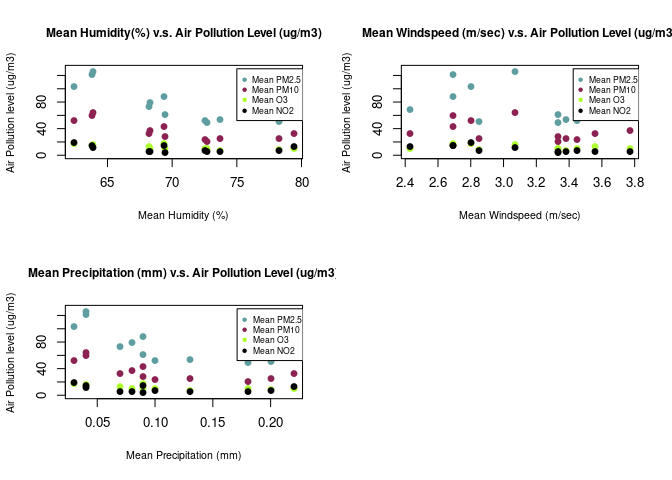
\includegraphics{Finalproject_files/figure-latex/unnamed-chunk-17-1.pdf}

From the result graph, what we can see is that the air pollution and
weather conditions seem to be in negative relationships. In other words,
with the increase of humidity/wind speed/precipitation, the air
pollution level will decrease. For average wind speed v.s. air pollution
level, their relationship is less clear. Therefore, I decide to make a
table to show each of the correlation coefficient and check the whether
the correlation coefficient matters scientifically. Hope there can be
something interesting.

\begin{Shaded}
\begin{Highlighting}[]
\NormalTok{ctbl }\OtherTok{\textless{}{-}} \FunctionTok{data.frame}\NormalTok{(}
  \AttributeTok{AQ\_Index =} \FunctionTok{c}\NormalTok{(}\StringTok{"PM2.5"}\NormalTok{,}\StringTok{"PM10"}\NormalTok{,}\StringTok{"O3"}\NormalTok{,}\StringTok{"NO2"}\NormalTok{), }
  \AttributeTok{Mean\_Humidity =} \FunctionTok{c}\NormalTok{(}\FunctionTok{cor}\NormalTok{(summary}\SpecialCharTok{$}\NormalTok{mean\_humidity,summary}\SpecialCharTok{$}\NormalTok{mean\_pm25),}\FunctionTok{cor}\NormalTok{(summary}\SpecialCharTok{$}\NormalTok{mean\_humidity,summary}\SpecialCharTok{$}\NormalTok{mean\_pm10),}\FunctionTok{cor}\NormalTok{(summary}\SpecialCharTok{$}\NormalTok{mean\_humidity,summary}\SpecialCharTok{$}\NormalTok{mean\_o3),}\FunctionTok{cor}\NormalTok{(summary}\SpecialCharTok{$}\NormalTok{mean\_humidity,summary}\SpecialCharTok{$}\NormalTok{mean\_no2)),}
  \AttributeTok{Mean\_Windspeed =} \FunctionTok{c}\NormalTok{(}\FunctionTok{cor}\NormalTok{(summary}\SpecialCharTok{$}\NormalTok{mean\_windspeed,summary}\SpecialCharTok{$}\NormalTok{mean\_pm25),}\FunctionTok{cor}\NormalTok{(summary}\SpecialCharTok{$}\NormalTok{mean\_windspeed,summary}\SpecialCharTok{$}\NormalTok{mean\_pm10),}\FunctionTok{cor}\NormalTok{(summary}\SpecialCharTok{$}\NormalTok{mean\_windspeed,summary}\SpecialCharTok{$}\NormalTok{mean\_o3),}\FunctionTok{cor}\NormalTok{(summary}\SpecialCharTok{$}\NormalTok{mean\_windspeed,summary}\SpecialCharTok{$}\NormalTok{mean\_no2)),}
  \AttributeTok{Mean\_Precipitation =} \FunctionTok{c}\NormalTok{(}\FunctionTok{cor}\NormalTok{(summary}\SpecialCharTok{$}\NormalTok{mean\_precipitation,summary}\SpecialCharTok{$}\NormalTok{mean\_pm25),}\FunctionTok{cor}\NormalTok{(summary}\SpecialCharTok{$}\NormalTok{mean\_precipitation,summary}\SpecialCharTok{$}\NormalTok{mean\_pm10),}\FunctionTok{cor}\NormalTok{(summary}\SpecialCharTok{$}\NormalTok{mean\_precipitation,summary}\SpecialCharTok{$}\NormalTok{mean\_o3),}\FunctionTok{cor}\NormalTok{(summary}\SpecialCharTok{$}\NormalTok{mean\_precipitation,summary}\SpecialCharTok{$}\NormalTok{mean\_no2))}
\NormalTok{  )}
\NormalTok{ctbl}
\end{Highlighting}
\end{Shaded}

\begin{verbatim}
##   AQ_Index Mean_Humidity Mean_Windspeed Mean_Precipitation
## 1    PM2.5    -0.7979218     -0.3633463         -0.7298353
## 2     PM10    -0.7748101     -0.3938262         -0.7065819
## 3       O3    -0.7662354     -0.3601008         -0.7171954
## 4      NO2    -0.4058509     -0.7878014         -0.3167795
\end{verbatim}

According to Pearson correlation coefficient rule{[}2{]}, when the
absolute value of r is greater than 0.7, then the relationship is
considered as strong; when the absolute value of r is greater than 0.5
but less than 0.7, the relationship is considered as moderate; when the
absolute value of r is greater than 0.3 but less than 0.5, then the
relationship is considered as weak; otherwise none or very weak
relationship. As we can see from the table, nearly half of the
relationships are statistically meaningful. The correlation coefficients
between PM2.5 and mean humidity, PM10 and mean humidity, O3 and mean
humidity, NO2 and mean wind speed, PM2.5 and precipitation, PM10 and
precipitation, and O3 and precipitation are larger than 0.7, which means
that they have a relatively strong relationship. The correlation
coefficients between mean humidity and NO2 and mean precipitation and
NO2 are among 0.3 to 0.5, which are considered as weak, and these
relationships verify the statement I made before that the water
contained in the air does not influence toxic air like NO2 much. An
interesting thing I found from the table is that, O3, also as toxic air,
has a strong relationship with mean humidity and mean precipitation. My
explanation is that O3 typically dissolve into water better than other
toxic air like NO2, so they are more impacted by the humidity and
precipitation level. In summary, the weather conditions are also one of
the factors which influence the air pollution level in Bangkok.

\#Summary

From this project, I successfully explore the factors behind the air
pollution in Bangkok. I have seen the socio-economic factors like the
construction of infrastructures and natural factors like the geography
and local weather conditions. They all play roles in the local air
quality. However, I also witness the environmental injustice in Bangkok,
and after searching on the internet, I do find many articles on the
desperation of local people about their unfair life conditions. Everyone
in every part of the world has the rights to enjoy clean air, water, or
space. I hope the local governments can take more feasible actions to
solve the local air quality and environment injustice issue in a
scientific and fair way, such as applying United Nations' 17 Sustainable
Development Goals into their daily work.

\#Reference:

{[}1{]}. Winn, Patrick. ``Bangkok: A City of Glitz, A City of
Desperation.'' World. npr. 2013.
\url{https://www.npr.org/2013/01/15/169439486/bangkok-a-city-of-glitz-a-city-of-desperation}

{[}2{]}. ``Correlation Coefficient: Simple Definition, Formula, Easy
Steps.'' Statistics How to. 2018.
\url{https://www.statisticshowto.com/probability-and-statistics/correlation-coefficient-formula/}

\end{document}
